% Font options: 10pm, 11pt, 12pt
% Align headings left instead of center: nocenter
\documentclass[xcolor=x11names,compress]{beamer}\usepackage[]{graphicx}\usepackage[]{color}
%% maxwidth is the original width if it is less than linewidth
%% otherwise use linewidth (to make sure the graphics do not exceed the margin)
\makeatletter
\def\maxwidth{ %
  \ifdim\Gin@nat@width>\linewidth
    \linewidth
  \else
    \Gin@nat@width
  \fi
}
\makeatother

\definecolor{fgcolor}{rgb}{0.345, 0.345, 0.345}
\newcommand{\hlnum}[1]{\textcolor[rgb]{0.686,0.059,0.569}{#1}}%
\newcommand{\hlstr}[1]{\textcolor[rgb]{0.192,0.494,0.8}{#1}}%
\newcommand{\hlcom}[1]{\textcolor[rgb]{0.678,0.584,0.686}{\textit{#1}}}%
\newcommand{\hlopt}[1]{\textcolor[rgb]{0,0,0}{#1}}%
\newcommand{\hlstd}[1]{\textcolor[rgb]{0.345,0.345,0.345}{#1}}%
\newcommand{\hlkwa}[1]{\textcolor[rgb]{0.161,0.373,0.58}{\textbf{#1}}}%
\newcommand{\hlkwb}[1]{\textcolor[rgb]{0.69,0.353,0.396}{#1}}%
\newcommand{\hlkwc}[1]{\textcolor[rgb]{0.333,0.667,0.333}{#1}}%
\newcommand{\hlkwd}[1]{\textcolor[rgb]{0.737,0.353,0.396}{\textbf{#1}}}%
\let\hlipl\hlkwb

\usepackage{framed}
\makeatletter
\newenvironment{kframe}{%
 \def\at@end@of@kframe{}%
 \ifinner\ifhmode%
  \def\at@end@of@kframe{\end{minipage}}%
  \begin{minipage}{\columnwidth}%
 \fi\fi%
 \def\FrameCommand##1{\hskip\@totalleftmargin \hskip-\fboxsep
 \colorbox{shadecolor}{##1}\hskip-\fboxsep
     % There is no \\@totalrightmargin, so:
     \hskip-\linewidth \hskip-\@totalleftmargin \hskip\columnwidth}%
 \MakeFramed {\advance\hsize-\width
   \@totalleftmargin\z@ \linewidth\hsize
   \@setminipage}}%
 {\par\unskip\endMakeFramed%
 \at@end@of@kframe}
\makeatother

\definecolor{shadecolor}{rgb}{.97, .97, .97}
\definecolor{messagecolor}{rgb}{0, 0, 0}
\definecolor{warningcolor}{rgb}{1, 0, 1}
\definecolor{errorcolor}{rgb}{1, 0, 0}
\newenvironment{knitrout}{}{} % an empty environment to be redefined in TeX

\usepackage{alltt}
%\documentclass[xcolor=x11names,compress,handout]{beamer}
\usepackage[]{graphicx}
\usepackage[]{color}
\usepackage{booktabs}
\usepackage{hyperref}
\usepackage{tikz}
\usepackage{multirow}
\usepackage{multicol}
\usepackage{dcolumn}
\usepackage{bigstrut}
\usepackage{amsmath} 
\usepackage{xcolor,colortbl}
\usepackage{amssymb}
%\newcommand{\done}{\cellcolor{teal}#1}

%% Beamer Layout %%%%%%%%%%%%%%%%%%%%%%%%%%%%%%%%%%
\useoutertheme[subsection=false,shadow]{miniframes}
\useinnertheme{default}
\usefonttheme{serif}
\usepackage{Arev}
\usepackage{pdfpages}

\setbeamerfont{title like}{shape=\scshape}
\setbeamerfont{frametitle}{shape=\scshape, size=\normalsize}

\definecolor{dkblue}{RGB}{0,0,102}

\setbeamercolor*{lower separation line head}{bg=dkblue} 
\setbeamercolor*{normal text}{fg=black,bg=white} 
\setbeamercolor*{alerted text}{fg=red} 
\setbeamercolor*{example text}{fg=black} 
\setbeamercolor*{structure}{fg=black} 
 
\setbeamercolor*{palette tertiary}{fg=black,bg=black!10} 
\setbeamercolor*{palette quaternary}{fg=black,bg=black!10} 

\renewcommand{\(}{\begin{columns}}
\renewcommand{\)}{\end{columns}}
\newcommand{\<}[1]{\begin{column}{#1}}
\renewcommand{\>}{\end{column}}

\setbeamertemplate{navigation symbols}{} 
\setbeamertemplate{footline}[frame number]
\setbeamertemplate{caption}{\raggedright\insertcaption\par}

\setbeamersize{text margin left=5pt,text margin right=5pt}

\AtBeginSection{\frame{\sectionpage}}
\usepackage{xcolor}
\hypersetup{
    colorlinks,
    linkcolor={red!50!black},
    citecolor={blue!50!black},
    urlcolor={blue!80!black}
}

%%%%%%%%%%%%%%%%%%%%%%%%%%%%%%%%%%%%%%%%%%%%%%%%%%







\title{FLS 6441 - Methods III: Explanation and Causation}
\subtitle{Week 1 - Review of Regression}
\author{Jonathan Phillips}
\date{February 2019}
\IfFileExists{upquote.sty}{\usepackage{upquote}}{}
\begin{document}

\frame{\titlepage}

\begin{frame}
\frametitle{Course Objectives}
\begin{enumerate}
\item Change how you think about quantitative methods, \textit{explaining} politics, and not just describing it
\item Understand the 'toolkit' of methods used in top journals
\item Apply those methods to your own research questions
\end{enumerate}
\begin{center}
\href{https://jonnyphillips.github.io/Methods_III}{Course Website}
\end{center}
\end{frame}

\begin{frame}
\frametitle{Course Topics}
\begin{enumerate}
\item Review of Regression
\item A Framework for Explanation
\item Field Experiments
\item Survey and Lab Experiments
\item Randomized Natural Experiments
\item Instrumental Variables
\item Discontinuities
\item Difference-in-Differences
\item Controlling for Confounding
\item Matching
\item Comparative Cases and Process Tracing
\item Generalizability, Reproducibility and Mechanisms
\end{enumerate}
\end{frame}

\begin{frame}
\frametitle{Course Schedule}
\begin{itemize}
\item Wednesday 18h - Submit Replication Task
\item Thursday 14h-16h - Class
\item Thursday 16.15-17.30 - Lab
\item Friday 10h-12h - Office Hours (DCP 2061)
\end{itemize}
\end{frame}

\begin{frame}
\frametitle{Project}
\begin{itemize}
\item Quality $>$ Quantity
\item Max 15 pages, English or Portuguese
\item Submit paper and code by email to me by 30th June 2019
\item Use at least one of the methods studied in class
\item Pick a simple question and dataset
\end{itemize}
\end{frame}

\begin{frame}
\frametitle{Today's Objectives}
\begin{enumerate}
\item What Does Regression Actually Do?
\item Guide to 'Smart' Regression
\item What Does Regression NOT Do?
\end{enumerate}
\end{frame}

\section{What Does Regression Actually Do?}

\begin{frame}
\frametitle{Data}
\begin{enumerate}
\item We work with variables, which VARY!
\end{enumerate}
\begin{multicols}{2}
% latex table generated in R 3.5.2 by xtable 1.8-3 package
% Sat Mar 02 10:50:44 2019
\begin{table}[ht]
\centering
\begin{tabular}{rr}
  \hline
 & Variable \\ 
  \hline
1 & 0.39 \\ 
  2 & 1.69 \\ 
  3 & -1.05 \\ 
  4 & -1.38 \\ 
  5 & 0.81 \\ 
  6 & 2.01 \\ 
  7 & 0.06 \\ 
  8 & 0.98 \\ 
  9 & -0.98 \\ 
  10 & -0.39 \\ 
   \hline
\end{tabular}
\end{table}

\columnbreak
\begin{knitrout}
\definecolor{shadecolor}{rgb}{0.969, 0.969, 0.969}\color{fgcolor}
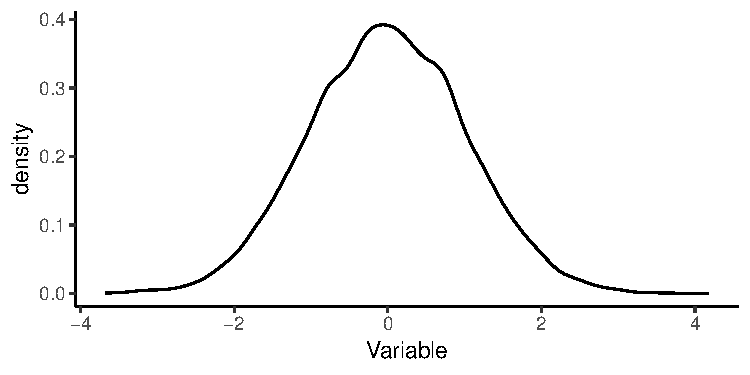
\includegraphics[width=\maxwidth]{figure/var2-1} 

\end{knitrout}
\end{multicols}
\end{frame}

% Bayes Rule: P(AnB)=P(A|B)*P(B)
% Independence: P(AnB)=P(A)*P(B) -> AIndepB. P(A|B)=P(A)
% E(x)=for random variable; (weighted) average is for sample. Same in large N/many repeated. Lecture 2, slide 69



\begin{frame}
\frametitle{What Does Regression Actually Do?}
\begin{enumerate}
\item Regression as Least Squares
\item Regression as Conditional Expectation
\item Regression as (Partial) Correlation
\end{enumerate}
\end{frame}


\begin{frame}
\frametitle{Regression as Least Squares}
\begin{itemize}
\item Regression identifies the line through the data that minimizes the sum of squared vertical distances 
\pause
\item $y_i = \alpha + \beta D_i + \epsilon_i$
\pause
\end{itemize}
\begin{multicols}{2}
Slope = 0
\begin{knitrout}
\definecolor{shadecolor}{rgb}{0.969, 0.969, 0.969}\color{fgcolor}
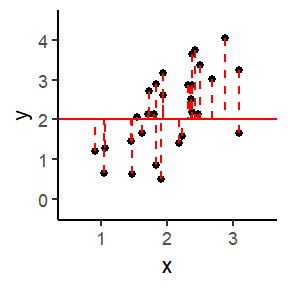
\includegraphics[width=\maxwidth]{figure/graph_ols1-1} 

\end{knitrout}
\columnbreak
Sum of Squared Residuals = 29.6
\begin{knitrout}
\definecolor{shadecolor}{rgb}{0.969, 0.969, 0.969}\color{fgcolor}
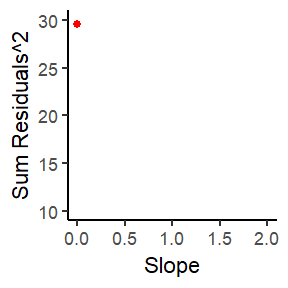
\includegraphics[width=\maxwidth]{figure/graph_ssr1-1} 

\end{knitrout}
\end{multicols}
\end{frame}

\begin{frame}
\frametitle{Regression as Least Squares}
\begin{itemize}
\item Regression identifies the line through the data that minimizes the sum of squared vertical distances 
\item $y_i = \alpha + \beta D_i + \epsilon_i$
\end{itemize}
\begin{multicols}{2}
Slope = 0.5
\begin{knitrout}
\definecolor{shadecolor}{rgb}{0.969, 0.969, 0.969}\color{fgcolor}
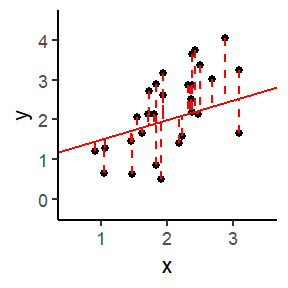
\includegraphics[width=\maxwidth]{figure/graph_ols2-1} 

\end{knitrout}
\columnbreak
Sum of Squared Residuals = 21.6
\begin{knitrout}
\definecolor{shadecolor}{rgb}{0.969, 0.969, 0.969}\color{fgcolor}
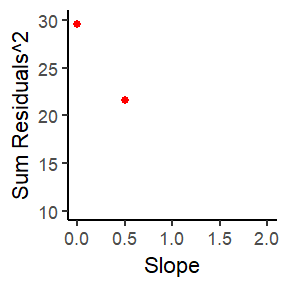
\includegraphics[width=\maxwidth]{figure/graph_ssr2-1} 

\end{knitrout}
\end{multicols}
\end{frame}

\begin{frame}
\frametitle{Regression as Least Squares}
\begin{itemize}
\item Regression identifies the line through the data that minimizes the sum of squared vertical distances 
\item $y_i = \alpha + \beta D_i + \epsilon_i$
\end{itemize}
\begin{multicols}{2}
Slope = 1
\begin{knitrout}
\definecolor{shadecolor}{rgb}{0.969, 0.969, 0.969}\color{fgcolor}
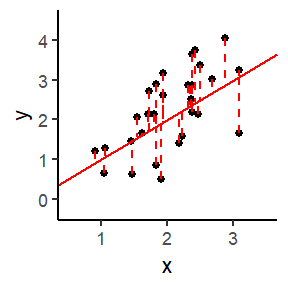
\includegraphics[width=\maxwidth]{figure/graph_ols3-1} 

\end{knitrout}
\columnbreak
Sum of Squared Residuals = 18.3
\begin{knitrout}
\definecolor{shadecolor}{rgb}{0.969, 0.969, 0.969}\color{fgcolor}
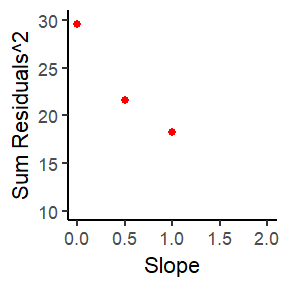
\includegraphics[width=\maxwidth]{figure/graph_ssr3-1} 

\end{knitrout}
\end{multicols}
\end{frame}

\begin{frame}
\frametitle{Regression as Least Squares}
\begin{itemize}
\item Regression identifies the line through the data that minimizes the sum of squared vertical distances 
\item $y_i = \alpha + \beta D_i + \epsilon_i$
\end{itemize}
\begin{multicols}{2}
Slope = 1.5
\begin{knitrout}
\definecolor{shadecolor}{rgb}{0.969, 0.969, 0.969}\color{fgcolor}
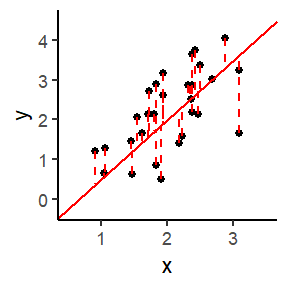
\includegraphics[width=\maxwidth]{figure/graph_ols4-1} 

\end{knitrout}
\columnbreak
Sum of Squared Residuals = 19.6
\begin{knitrout}
\definecolor{shadecolor}{rgb}{0.969, 0.969, 0.969}\color{fgcolor}
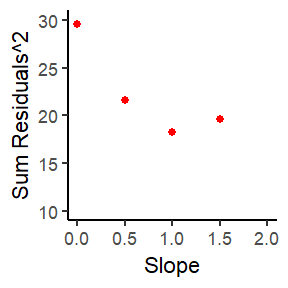
\includegraphics[width=\maxwidth]{figure/graph_ssr4-1} 

\end{knitrout}
\end{multicols}
\end{frame}

\begin{frame}
\frametitle{Regression as Least Squares}
\begin{itemize}
\item Regression identifies the line through the data that minimizes the sum of squared vertical distances 
\item $y_i = \alpha + \beta D_i + \epsilon_i$
\end{itemize}
\begin{multicols}{2}
Slope = 2
\begin{knitrout}
\definecolor{shadecolor}{rgb}{0.969, 0.969, 0.969}\color{fgcolor}
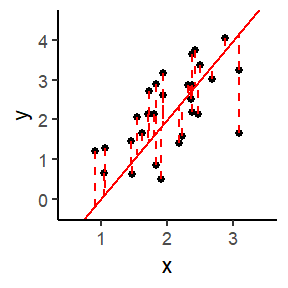
\includegraphics[width=\maxwidth]{figure/graph_ols5-1} 

\end{knitrout}
\columnbreak
Sum of Squared Residuals = 25.5
\begin{knitrout}
\definecolor{shadecolor}{rgb}{0.969, 0.969, 0.969}\color{fgcolor}
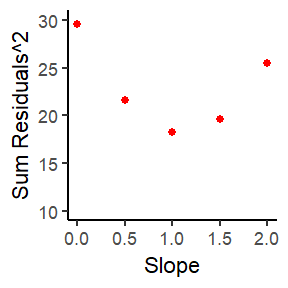
\includegraphics[width=\maxwidth]{figure/graph_ssr5-1} 

\end{knitrout}
\end{multicols}
\end{frame}

\begin{frame}
\frametitle{Regression as Least Squares}
\begin{itemize}
\item Regression identifies the line through the data that minimizes the sum of squared vertical distances 
\item $y_i = \alpha + \beta D_i + \epsilon_i$
\end{itemize}
\begin{multicols}{2}
Slope = 1
\begin{knitrout}
\definecolor{shadecolor}{rgb}{0.969, 0.969, 0.969}\color{fgcolor}
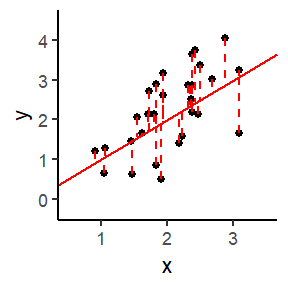
\includegraphics[width=\maxwidth]{figure/graph_ols6-1} 

\end{knitrout}
\columnbreak
Sum of Squared Residuals = 18.3
\begin{knitrout}
\definecolor{shadecolor}{rgb}{0.969, 0.969, 0.969}\color{fgcolor}
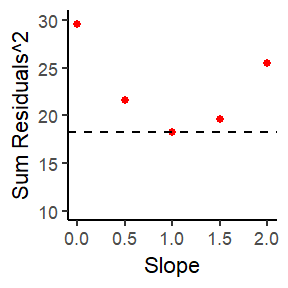
\includegraphics[width=\maxwidth]{figure/graph_ssr6-1} 

\end{knitrout}
\end{multicols}
\end{frame}

%Add noise
\begin{frame}
\frametitle{Regression as Least Squares}
\begin{itemize}
\item If we add pure \textit{noise} to $y$, our estimate of $\beta$ is unchanged
\begin{itemize}
\item The residual error increases
\end{itemize}
\item $y_i = \alpha + \beta D_i + \epsilon_i$
\end{itemize}
\begin{multicols}{2}
Slope = 1
\begin{knitrout}
\definecolor{shadecolor}{rgb}{0.969, 0.969, 0.969}\color{fgcolor}
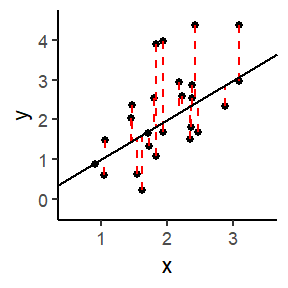
\includegraphics[width=\maxwidth]{figure/graph_ols7-1} 

\end{knitrout}
\columnbreak
Sum of Squared Residuals = 63.9
\begin{knitrout}
\definecolor{shadecolor}{rgb}{0.969, 0.969, 0.969}\color{fgcolor}
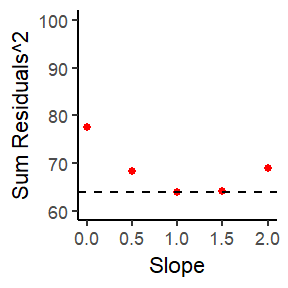
\includegraphics[width=\maxwidth]{figure/graph_ssr7-1} 

\end{knitrout}
\end{multicols}
\end{frame}

\begin{frame}
\frametitle{Regression as Least Squares}
\begin{itemize}
\item Dummy control variables \textit{remove variation} associated with specific levels or categories
\begin{itemize}
\item The same for fixed effects
\end{itemize}
\item $y_{ij} = \alpha + \beta_1 D_{ij} + \epsilon_i$
\end{itemize}
\begin{multicols}{2}
\begin{knitrout}
\definecolor{shadecolor}{rgb}{0.969, 0.969, 0.969}\color{fgcolor}
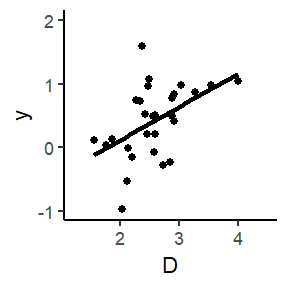
\includegraphics[width=\maxwidth]{figure/graph_ols_FE1-1} 

\end{knitrout}
\columnbreak
Ignoring the dummy control variable, the slope coefficient is 1 
\end{multicols}
\end{frame}

\begin{frame}
\frametitle{Regression as Least Squares}
\begin{itemize}
\item Dummy control variables \textit{remove variation} associated with specific levels or categories
\begin{itemize}
\item The same for fixed effects
\end{itemize}
\item $y_{ij} = \alpha + \beta_1 D_{ij} + \epsilon_i$
\end{itemize}
\begin{multicols}{2}
\begin{knitrout}
\definecolor{shadecolor}{rgb}{0.969, 0.969, 0.969}\color{fgcolor}
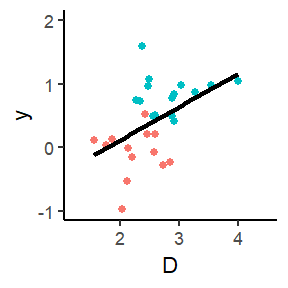
\includegraphics[width=\maxwidth]{figure/graph_ols_FE2-1} 

\end{knitrout}
\columnbreak
But the data points really represent two very different groups, blues and reds
\end{multicols}
\end{frame}

\begin{frame}
\frametitle{Regression as Least Squares}
\begin{itemize}
\item Dummy control variables \textit{remove variation} associated with specific levels or categories
\begin{itemize}
\item The same for fixed effects
\end{itemize}
\item $y_{ij} = \alpha + \beta_1 D_{ij} + \beta_2 X_j + \epsilon_i$
\end{itemize}
\begin{multicols}{2}
\begin{knitrout}
\definecolor{shadecolor}{rgb}{0.969, 0.969, 0.969}\color{fgcolor}
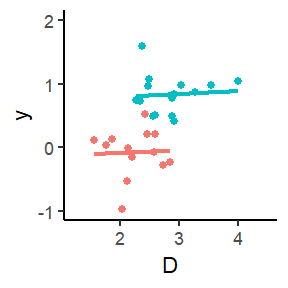
\includegraphics[width=\maxwidth]{figure/graph_ols_FE3-1} 

\end{knitrout}
\columnbreak
What if we treated each group \textit{separately}?
\end{multicols}
\end{frame}

\begin{frame}
\frametitle{Regression as Least Squares}
\begin{itemize}
\item Dummy control variables \textit{remove variation} associated with specific levels or categories
\begin{itemize}
\item The same for fixed effects
\end{itemize}
\item $y_{ij} = \alpha + \beta_1 D_{ij} + \beta_2 X_j + \epsilon_i$
\end{itemize}
\begin{multicols}{2}
\begin{knitrout}
\definecolor{shadecolor}{rgb}{0.969, 0.969, 0.969}\color{fgcolor}
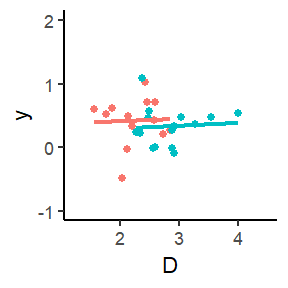
\includegraphics[width=\maxwidth]{figure/graph_ols_FE4-1} 

\end{knitrout}
\columnbreak
Dummy control variables \textit{remove} the average $Y$ differences between blues and reds
\end{multicols}
\end{frame}

\begin{frame}
\frametitle{Regression as Least Squares}
\begin{itemize}
\item Dummy control variables \textit{remove variation} associated with specific levels or categories
\begin{itemize}
\item The same for fixed effects
\end{itemize}
\item $y_{ij} = \alpha + \beta_1 D_{ij} + \beta_2 X_j + \epsilon_i$
\end{itemize}
\begin{multicols}{2}
\begin{knitrout}
\definecolor{shadecolor}{rgb}{0.969, 0.969, 0.969}\color{fgcolor}
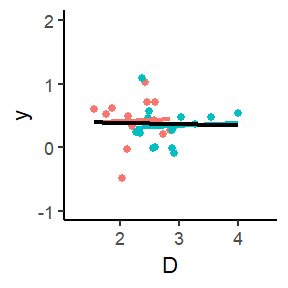
\includegraphics[width=\maxwidth]{figure/graph_ols_FE5-1} 

\end{knitrout}
\columnbreak
The new regression line for the full data now has a slope of zero
\end{multicols}
\end{frame}

\begin{frame}
\frametitle{Regression as Least Squares}
\begin{itemize}
\item Dummy control variables \textit{remove variation} associated with specific levels or categories
\begin{itemize}
\item The same for fixed effects
\end{itemize}
\item $y_{ij} = \alpha + \beta_1 D_{ij} + \beta_2 X_j + \epsilon_i$
\end{itemize}
\begin{multicols}{2}
\begin{knitrout}
\definecolor{shadecolor}{rgb}{0.969, 0.969, 0.969}\color{fgcolor}
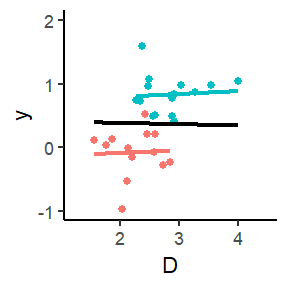
\includegraphics[width=\maxwidth]{figure/graph_ols_FE_last-1} 

\end{knitrout}
\columnbreak
\footnotesize
Equivalently, dummy control variables restrict comparisons to \textbf{within the same group}:
\begin{enumerate}
\item How much does $X$ affect $Y$ within the blue group? Zero
\item How much does $X$ affect $Y$ within the red group? Zero
\item What's the average of (1) and (2) (weighted by the number of units in each group)? Zero
\normalsize
\end{enumerate}
\end{multicols}
\end{frame}

\begin{frame}
\frametitle{Regression as Least Squares}
\begin{itemize}
\item Continuous control variables \textit{remove variation} based on how much the control explains $y$
\item $y_i = \alpha + \beta_1 D_i + \epsilon_i$
\end{itemize}
\begin{multicols}{2}
\begin{knitrout}
\definecolor{shadecolor}{rgb}{0.969, 0.969, 0.969}\color{fgcolor}
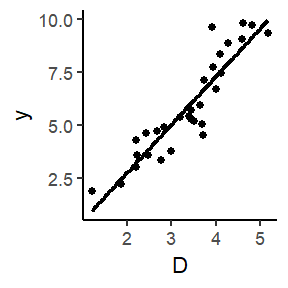
\includegraphics[width=\maxwidth]{figure/graph_ols_control1-1} 

\end{knitrout}
\columnbreak

The coefficient $\beta_1$ is 2.267 \\
Real effect = 1
\end{multicols}
\end{frame}

\begin{frame}
\frametitle{Regression as Least Squares}
\begin{itemize}
\item Continuous control variables \textit{remove variation} based on how much the control explains $y$
\item $y_i = \alpha + \beta_1 D_i + \epsilon_i$
\end{itemize}
\begin{multicols}{2}
\begin{knitrout}
\definecolor{shadecolor}{rgb}{0.969, 0.969, 0.969}\color{fgcolor}
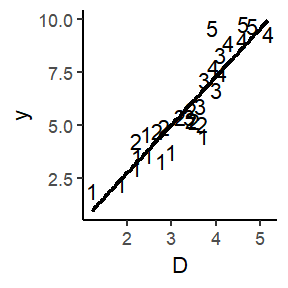
\includegraphics[width=\maxwidth]{figure/graph_ols_control2-1} 

\end{knitrout}
\columnbreak
The coefficient $\beta_1$ is 2.267 \\
Real effect = 1
\end{multicols}
\end{frame}

\begin{frame}
\frametitle{Regression as Least Squares}
\begin{itemize}
\item Continuous control variables \textit{remove variation} based on how much the control explains $y$
\item $y_i = \alpha + \beta_1 D_i + \beta_2 X_i + \epsilon_i$
\end{itemize}
\begin{multicols}{2}
\begin{knitrout}
\definecolor{shadecolor}{rgb}{0.969, 0.969, 0.969}\color{fgcolor}
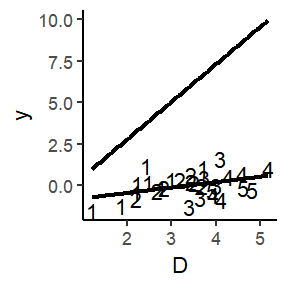
\includegraphics[width=\maxwidth]{figure/graph_ols_control3-1} 

\end{knitrout}
\columnbreak

The coefficient $\beta_1$ is 1.024 \\
Real effect = 1
\end{multicols}
\end{frame}

\begin{frame}
\frametitle{Regression as Conditional Expectation}
\begin{itemize}
\item Regression is also a \textbf{Conditional Expectation Function}
\pause
\item Conditional on $x$, what is our expectation (mean value) of $y$?
\end{itemize}
\begin{center}
\item $y_i = \alpha + \beta_1 D_i + \epsilon_i$
\pause
\item $Attitude_i = \alpha + \beta_1 Income_i + N(0,\sigma^2)$
\pause
\item $Attitude_i = 2.235 - 0.000818 * Income_i + N(0,2.38)$
\pause
\end{center}
\begin{itemize}
\item $E(y|x)$, \pause  $E(Attitude | Income)$
\begin{itemize}
\item When income is 3000, the average attitude is -0.22
\item When income  is 6000, the average attitude is -2.67
\end{itemize}
\item $E(attitude|income,age,gender,municipality)$
\end{itemize}
\end{frame}

\begin{frame}
\frametitle{Regression as Conditional Expectation}
\begin{knitrout}
\definecolor{shadecolor}{rgb}{0.969, 0.969, 0.969}\color{fgcolor}
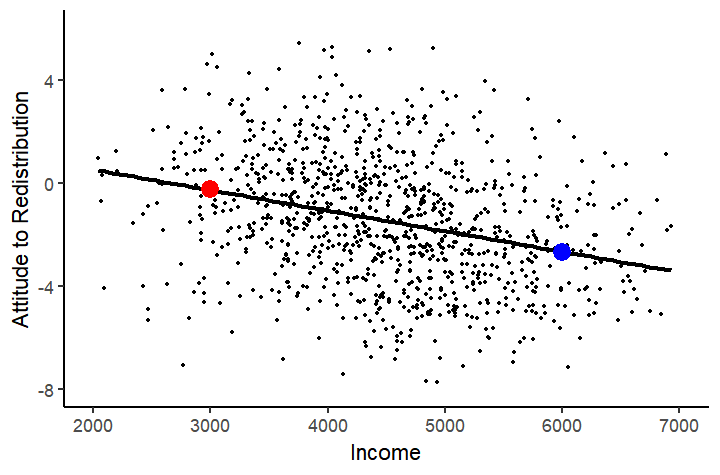
\includegraphics[width=\maxwidth]{figure/cond_exp1-1} 

\end{knitrout}
\end{frame}

\begin{frame}
\frametitle{Regression as Conditional Expectation}
\begin{knitrout}
\definecolor{shadecolor}{rgb}{0.969, 0.969, 0.969}\color{fgcolor}
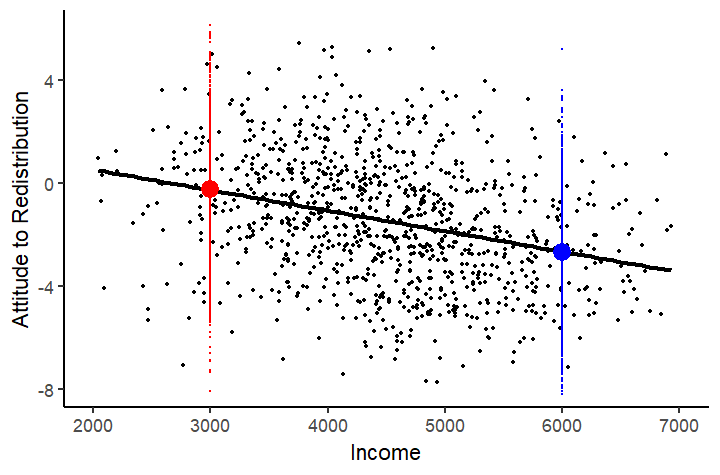
\includegraphics[width=\maxwidth]{figure/cond_exp1b-1} 

\end{knitrout}
\end{frame}

\begin{frame}
\frametitle{Regression as Conditional Expectation}
\begin{itemize}
\item How do we work out the conditional expectation? We estimate $\beta$
\pause
\item But we \textbf{NEVER} know the exact value of $\beta$
\pause
\item Regression \textbf{estimates a distribution} for $\beta$
\pause
\begin{itemize}
\item That's why every $\beta$ comes with a standard error
\pause
\end{itemize}
\end{itemize}
\begin{multicols}{2}

% Table created by stargazer v.5.2.2 by Marek Hlavac, Harvard University. E-mail: hlavac at fas.harvard.edu
% Date and time: Thu, Mar 07, 2019 - 12:50:31 PM
\begin{table}[!htbp] \centering 
  \caption{} 
  \label{} 
\tiny 
\begin{tabular}{@{\extracolsep{1pt}}lc} 
\\[-1.8ex]\hline 
\hline \\[-1.8ex] 
 & \multicolumn{1}{c}{\textit{Dependent variable:}} \\ 
\cline{2-2} 
\\[-1.8ex] & redist \\ 
\hline \\[-1.8ex] 
 income & $-$0.000818$^{***}$ (0.000078) \\ 
  Constant & 2.234719$^{***}$ (0.361477) \\ 
 \hline \\[-1.8ex] 
Observations & 1,000 \\ 
\hline 
\hline \\[-1.8ex] 
\textit{Note:}  & \multicolumn{1}{r}{$^{*}$p$<$0.1; $^{**}$p$<$0.05; $^{***}$p$<$0.01} \\ 
\end{tabular} 
\end{table} 

\columnbreak
\begin{knitrout}
\definecolor{shadecolor}{rgb}{0.969, 0.969, 0.969}\color{fgcolor}
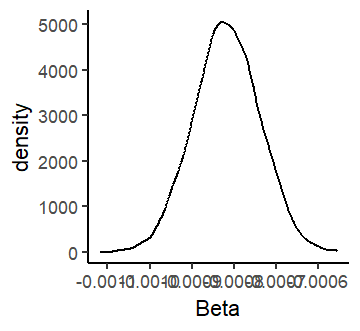
\includegraphics[width=\maxwidth]{figure/beta_dist-1} 

\end{knitrout}
\end{multicols}
\end{frame}

\begin{frame}
\frametitle{Regression as Conditional Expectation}
\begin{itemize}
\item How do we work out the conditional expectation? We estimate $\beta$
\item But we \textbf{NEVER} know the exact value of $\beta$
\item Regression \textbf{estimates a distribution} for $\beta$
\begin{itemize}
\item That's why every $\beta$ comes with a standard error
\end{itemize}
\end{itemize}
\begin{multicols}{2}

% Table created by stargazer v.5.2.2 by Marek Hlavac, Harvard University. E-mail: hlavac at fas.harvard.edu
% Date and time: Thu, Mar 07, 2019 - 1:07:24 PM
\begin{table}[!htbp] \centering 
  \caption{} 
  \label{} 
\tiny 
\begin{tabular}{@{\extracolsep{1pt}}lc} 
\\[-1.8ex]\hline 
\hline \\[-1.8ex] 
 & \multicolumn{1}{c}{\textit{Dependent variable:}} \\ 
\cline{2-2} 
\\[-1.8ex] & redist \\ 
\hline \\[-1.8ex] 
 income & $-$0.000818$^{***}$ (0.000078) \\ 
  Constant & 2.234719$^{***}$ (0.361477) \\ 
 \hline \\[-1.8ex] 
Observations & 1,000 \\ 
\hline 
\hline \\[-1.8ex] 
\textit{Note:}  & \multicolumn{1}{r}{$^{*}$p$<$0.1; $^{**}$p$<$0.05; $^{***}$p$<$0.01} \\ 
\end{tabular} 
\end{table} 

\columnbreak
\begin{knitrout}
\definecolor{shadecolor}{rgb}{0.969, 0.969, 0.969}\color{fgcolor}
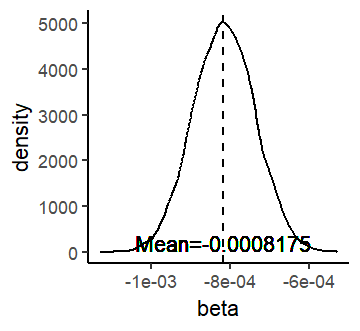
\includegraphics[width=\maxwidth]{figure/beta_dist_2-1} 

\end{knitrout}
\end{multicols}
\end{frame}

\begin{frame}
\frametitle{Regression as Conditional Expectation}
\begin{itemize}
\item How do we work out the conditional expectation? We estimate $\beta$
\item But we \textbf{NEVER} know the exact value of $\beta$
\item Regression \textbf{estimates a distribution} for $\beta$
\begin{itemize}
\item That's why every $\beta$ comes with a standard error
\end{itemize}
\end{itemize}
\begin{multicols}{2}

% Table created by stargazer v.5.2.2 by Marek Hlavac, Harvard University. E-mail: hlavac at fas.harvard.edu
% Date and time: Thu, Mar 07, 2019 - 1:07:27 PM
\begin{table}[!htbp] \centering 
  \caption{} 
  \label{} 
\tiny 
\begin{tabular}{@{\extracolsep{1pt}}lc} 
\\[-1.8ex]\hline 
\hline \\[-1.8ex] 
 & \multicolumn{1}{c}{\textit{Dependent variable:}} \\ 
\cline{2-2} 
\\[-1.8ex] & redist \\ 
\hline \\[-1.8ex] 
 income & $-$0.000818$^{***}$ (0.000078) \\ 
  Constant & 2.234719$^{***}$ (0.361477) \\ 
 \hline \\[-1.8ex] 
Observations & 1,000 \\ 
\hline 
\hline \\[-1.8ex] 
\textit{Note:}  & \multicolumn{1}{r}{$^{*}$p$<$0.1; $^{**}$p$<$0.05; $^{***}$p$<$0.01} \\ 
\end{tabular} 
\end{table} 

\columnbreak
\begin{knitrout}
\definecolor{shadecolor}{rgb}{0.969, 0.969, 0.969}\color{fgcolor}
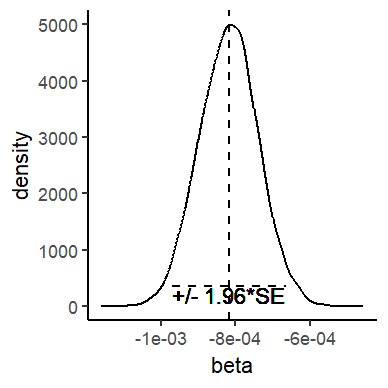
\includegraphics[width=\maxwidth]{figure/beta_dist_3-1} 

\end{knitrout}
\end{multicols}
\end{frame}

\begin{frame}
\frametitle{Regression as Conditional Expectation}
\begin{itemize}
\item How do we work out the conditional expectation? We estimate $\beta$
\item But we \textbf{NEVER} know the exact value of $\beta$
\item Regression \textbf{estimates a distribution} for $\beta$
\begin{itemize}
\item That's why every $\beta$ comes with a standard error
\end{itemize}
\end{itemize}
\begin{multicols}{2}

% Table created by stargazer v.5.2.2 by Marek Hlavac, Harvard University. E-mail: hlavac at fas.harvard.edu
% Date and time: Thu, Mar 07, 2019 - 1:07:32 PM
\begin{table}[!htbp] \centering 
  \caption{} 
  \label{} 
\tiny 
\begin{tabular}{@{\extracolsep{1pt}}lc} 
\\[-1.8ex]\hline 
\hline \\[-1.8ex] 
 & \multicolumn{1}{c}{\textit{Dependent variable:}} \\ 
\cline{2-2} 
\\[-1.8ex] & redist \\ 
\hline \\[-1.8ex] 
 income & $-$0.000818$^{***}$ (0.000078) \\ 
  Constant & 2.234719$^{***}$ (0.361477) \\ 
 \hline \\[-1.8ex] 
Observations & 1,000 \\ 
\hline 
\hline \\[-1.8ex] 
\textit{Note:}  & \multicolumn{1}{r}{$^{*}$p$<$0.1; $^{**}$p$<$0.05; $^{***}$p$<$0.01} \\ 
\end{tabular} 
\end{table} 

\columnbreak
\begin{knitrout}
\definecolor{shadecolor}{rgb}{0.969, 0.969, 0.969}\color{fgcolor}
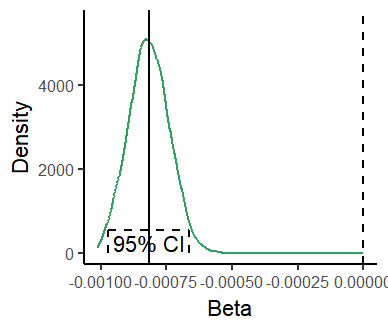
\includegraphics[width=\maxwidth]{figure/beta_dist_4-1} 

\end{knitrout}
\end{multicols}
\end{frame}



\begin{frame}
\frametitle{Regression as (Partial) Correlation}
\begin{itemize}
\item Regression with two variables is very similar to calculating correlation
\pause
\item $\hat{\beta}=cor(x,y) * \frac{\sigma_Y}{\sigma_X}$
\pause
\end{itemize}
\begin{multicols}{2}
\begin{knitrout}
\definecolor{shadecolor}{rgb}{0.969, 0.969, 0.969}\color{fgcolor}
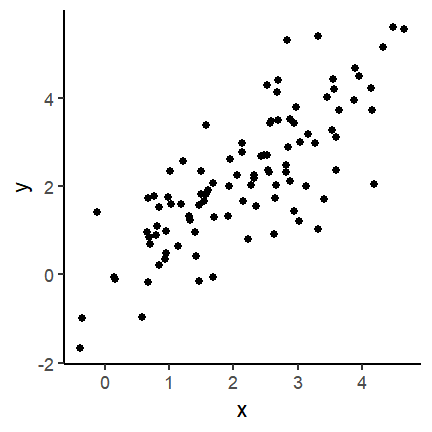
\includegraphics[width=\maxwidth]{figure/corr_regn_fig1-1} 

\end{knitrout}
\columnbreak
\end{multicols}
\end{frame}

\begin{frame}
\frametitle{Regression as (Partial) Correlation}
\begin{itemize}
\item Regression with two variables is very similar to calculating correlation:
\item $\hat{\beta}=cor(x,y) * \frac{\sigma_Y}{\sigma_X}$
\end{itemize}
\begin{multicols}{2}
\begin{knitrout}
\definecolor{shadecolor}{rgb}{0.969, 0.969, 0.969}\color{fgcolor}
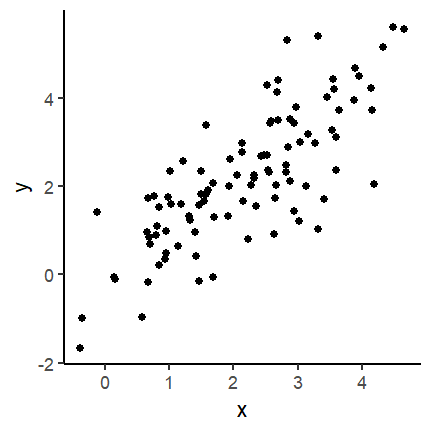
\includegraphics[width=\maxwidth]{figure/corr_regn_fig2-1} 

\end{knitrout}
\columnbreak
\begin{itemize}
\item Correlation is 0.781
\pause
\item Regression Results:
\end{itemize}
% latex table generated in R 3.5.2 by xtable 1.8-3 package
% Sat Mar 02 10:51:08 2019
\begin{table}[ht]
\centering
\begin{tabular}{rlr}
  \hline
 & term & estimate \\ 
  \hline
1 & (Intercept) & 0.006 \\ 
  2 & x & 1.008 \\ 
   \hline
\end{tabular}
\end{table}

\end{multicols}
\end{frame}

\begin{frame}
\frametitle{Regression as (Partial) Correlation}
\begin{itemize}
\item Regression with two variables is very similar to calculating correlation:
\item $\hat{\beta}=cor(x,y) * \frac{\sigma_Y}{\sigma_X}$
\end{itemize}
\begin{multicols}{2}
\begin{knitrout}
\definecolor{shadecolor}{rgb}{0.969, 0.969, 0.969}\color{fgcolor}
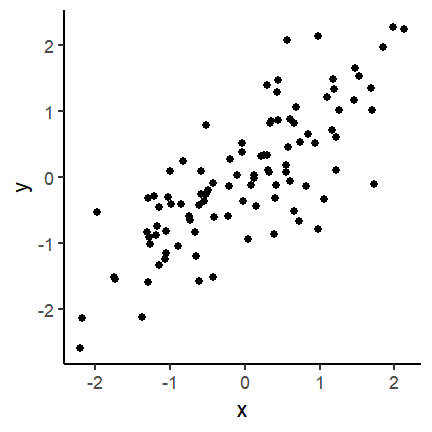
\includegraphics[width=\maxwidth]{figure/corr_regn_fig3-1} 

\end{knitrout}
\columnbreak
\begin{itemize}
\item It's \textit{identical} if we standardize both variables first ($\frac{(x-\bar{x})}{\sigma_x}$)
\item Correlation is 0.781
\item Standardized Regression Results:
\end{itemize}
% latex table generated in R 3.5.2 by xtable 1.8-3 package
% Sat Mar 02 10:51:11 2019
\begin{table}[ht]
\centering
\begin{tabular}{rlr}
  \hline
 & term & estimate \\ 
  \hline
1 & (Intercept) & 0.000 \\ 
  2 & x & 0.781 \\ 
   \hline
\end{tabular}
\end{table}

\end{multicols}
\end{frame}

\begin{frame}
\frametitle{Regression as (Partial) Correlation}
\begin{itemize}
\item Regression with \textbf{multiple} variables is very similar to calculating \textbf{partial} correlation
\pause
\item $y_i = \alpha + \beta_1 x_1 + \beta_2 x_2 +\epsilon_i$
\pause
\item Just a small difference in the denominator (how we standardize the measure)
\pause
\end{itemize}
$$\beta_{x_1} = \frac{r_{yx_1} - r_{yx_2}r_{x_1x_2}}{1-r^2_{x_1x_2}}$$
$$r_{yx_1|x_2} = \frac{r_{yx_1} - r_{yx_2}r_{x_1x_2}}{\sqrt{(1-r^2_{yx_2})(1-r^2_{x_1x_2})}}$$
\begin{itemize}
\item \textbf{There is no magic in regression, it's just 'extra' correlation}
\end{itemize}
\end{frame}



\section{Guide to 'Smart' Regression}

\begin{frame}
\frametitle{Regression Guide}
\begin{enumerate}
\item We will use regression throughout this course
\pause
\item But in a very \textbf{precise} way for each methodology
\pause
\item There are fundamental best practices that apply to all the methodologies
\end{enumerate}
\end{frame}

\begin{frame}
\frametitle{Regression Guide}
\begin{enumerate}
\item \textbf{Choose Variables and Measures:} To test a specific hypothesis
\pause
\item \textbf{Choose a Model/Link Function:} To match the data type of your outcome variable
\pause
\item \textbf{Choose Covariates:} To match your strategy of inference
\pause
\item \textbf{Choose Fixed Effects:} To focus on comparisons at a specific level
\pause
\item \textbf{Choose Error Structure:} To match known dependencies/clustering in the data or sampling
\pause
\item \textbf{Interpret the Coefficients:} To match the type/scale of the explanatory variable, outcome variable and model
\pause
\item \textbf{Predict Meaningful Comparisons:} To communicate your findings
\end{enumerate}
\end{frame}

\begin{frame}
\frametitle{1. Variables and Measures}
\begin{itemize}
\item For the research question ``Does income affect attitudes to redistribution?''
\pause
\item What measure of income should we use?
\pause
\begin{itemize}
\item Pre-tax, post-tax, after government benefits?
\end{itemize}
\item It depends on the theory we are testing
\end{itemize}
\end{frame}

\begin{frame}
\frametitle{2. Regression Models}
The Regression Model reflects the data type of the outcome variable:
\begin{itemize}
\item Continuous -> Ordinary Least Squares  
\begin{itemize}
\item Pick a precise number that reflects your attitude to redistribution
\end{itemize}
\item Binary -> Logit  
\begin{itemize}
\item Do you support redistribution, yes or no?
\end{itemize}
\item Unordered categories -> Multinomial logit  
\begin{itemize}
\item Do you think redistribution is a western, oriental or african concept?
\end{itemize}
\item Ordered categories -> Ordered logit  
\begin{itemize}
\item Do you want a lot more, more, the same, less, or a lot less redistribution?
\end{itemize}
\item Count -> Poisson  
\begin{itemize}
\item In the past year, how many times have you complained about redistribution?
\end{itemize}
\end{itemize}
\end{frame}

\begin{frame}
\frametitle{3. Covariates}
\begin{itemize}
\item Which covariates should we include?
\pause
\item Which comparisons do we want to make?
\pause
\item Control for gender if we want to compare men with men, women with women
\pause
\item Most crucial where there is theory or evidence that this variable could be an \textbf{omitted variable}
\end{itemize}
\end{frame}

\begin{frame}
\frametitle{4. Fixed Effects}
\begin{itemize}
\item Data are usually hierarchical: countries, states, municipalities, neighbourhoods, families, individuals
\pause
\item A fixed effect for countries means we only compare people within the same country
\pause
\item Removing \textit{ALL} the variation between countries
\begin{itemize}
\item If rich countries have stronger attitudes to redistribution, we control for this
\end{itemize}
\pause
\item Our question becomes: How do variations within income in the same country affect attitudes to redistribution?
\end{itemize}
\end{frame}

\begin{frame}
\frametitle{5. Errors Structure}
\begin{itemize}
\item After all of our controls and fixed effects, we need to think about the errors - the bit we cannot explain
\pause
\item An assumption of regression analysis is that the errors are independent
\begin{itemize}
\item Knowing the value of one error tells you \textit{nothing} about the value of the next error
\end{itemize}
\item But your attitudes to redistribution are probably very similar to everyone you live with, even after controlling for income etc.
\pause
\item So we don't really have 2 observations, we have closer to 1 'independent' observation
\item So the standard errors for our $\beta$'s are \textit{over-optimistic} (too small)
\pause
\item We need to adjust for these dependencies with clustered standard errors
\begin{itemize}
\item Created by the underlying structure of the data
\item Or by our data sampling process
\end{itemize}
\end{itemize}
\end{frame}

\begin{frame}
\frametitle{5. Errors Structure}
\begin{knitrout}
\definecolor{shadecolor}{rgb}{0.969, 0.969, 0.969}\color{fgcolor}
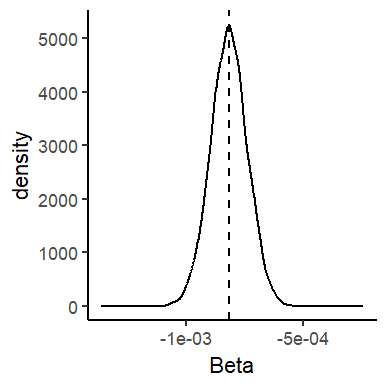
\includegraphics[width=\maxwidth]{figure/beta_dist_errors_4-1} 

\end{knitrout}
\end{frame}

\begin{frame}
\frametitle{6. Interpreting Regression Results}
\begin{itemize}
\item Difficult! It depends on the scale of the explanatory variable, scale of the outcome, the regression model we used, and the presence of any interaction
\item Basic OLS:
\begin{itemize}
\item 1 [unit of explanatory variable] change in the explanatory variable is associated with a $\beta$ [unit of outcome variable] change in the outcome
\end{itemize}
\end{itemize}
\end{frame}

\begin{frame}
\frametitle{6. Interpreting Regression Results}
\begin{itemize}
\item Difficult! It depends on the scale of the explanatory variable, scale of the outcome, the regression model we used, and the presence of any interaction
\item Logit:
\begin{itemize}
\item 1 [unit of explanatory variable] change in the explanatory variable is associated with a $\beta$ [unit of outcome variable] change in the outcome
\end{itemize}
\end{itemize}
\end{frame}

\begin{frame}
\frametitle{7. Predictions from Regressions}
\begin{itemize}
\item The coefficient on the regression of income on attitude to redistribution is -0.000818
\begin{itemize}
\pause
\item So??? What do we learn from this?
\pause
\item Coefficients are hard to interpret, and depend on how we measure each variable
\item And p-values are arbitrary
\end{itemize}  
\pause
\item Better to make specific \textit{predictions} of how changes in $X$ produce changes in $Y$
\end{itemize}
\end{frame}

\begin{frame}
\frametitle{7. Predictions from Regressions}
$$Attitude_i = \alpha + \beta_1 \text{ Income}_i + \epsilon_i$$ \\
\pause
$$Attitude_i = 2.235 - 0.000818 \text{ Income}_i + N(0,2.378)$$ \\
\pause
\textbf{If Income is 3000:}  \\
$$Attitude_i = 2.235-0.000818*3000 + N(0,2.378)$$ \\
$$Attitude_i = -0.219 + N(0,2.378)$$
\end{frame}

\begin{frame}
\frametitle{7. Predictions from Regressions}
$$Attitude_i = \alpha + \beta_1 \text{ Income}_i + \epsilon_i$$ \\
$$Attitude_i = 2.235 - 0.000818 \text{ Income}_i + N(0,2.378)$$ \\
\textbf{If Income is 6000:}  \\
$$Attitude_i = 2.235-0.000818*6000 + N(0,2.378)$$ \\
$$Attitude_i = -2.673 + N(0,2.378)$$
\end{frame}

\begin{frame}
\frametitle{7. Predictions from Regressions}
$$Attitude_i = \alpha + \beta_1 \text{ Income}_i + \epsilon_i$$
$$Attitude_i = 2.235 - 0.000818 \text{ Income}i + N(0,2.378)$$
\textbf{Increasing Income from 3000 to 6000:} \\
$$\Delta Attitude_i = (2.235-0.000818*6000) - (2.235-0.000818*3000)$$
$$\Delta Attitude_i = -2.673 - -0.219$$
$$\Delta Attitude_i = -2.454$$
\end{frame}

\begin{frame}
\frametitle{7. Predictions from Regressions}
\begin{knitrout}
\definecolor{shadecolor}{rgb}{0.969, 0.969, 0.969}\color{fgcolor}
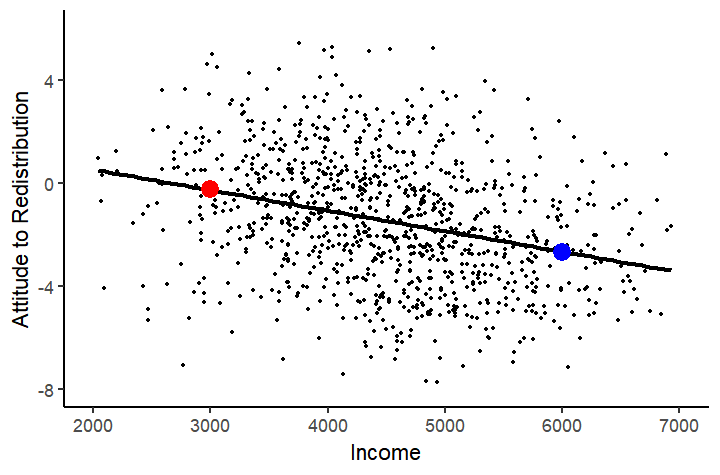
\includegraphics[width=\maxwidth]{figure/predictions1-1} 

\end{knitrout}
\end{frame}

\begin{frame}
\frametitle{7. Predictions from Regressions}
\begin{multicols}{2}
Predicted Values:
\begin{knitrout}
\definecolor{shadecolor}{rgb}{0.969, 0.969, 0.969}\color{fgcolor}
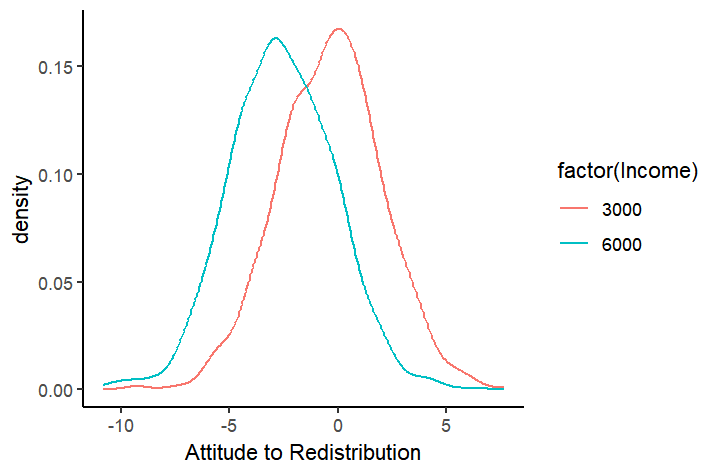
\includegraphics[width=\maxwidth]{figure/predictions2-1} 

\end{knitrout}
\columnbreak
First Differences:
\begin{knitrout}
\definecolor{shadecolor}{rgb}{0.969, 0.969, 0.969}\color{fgcolor}
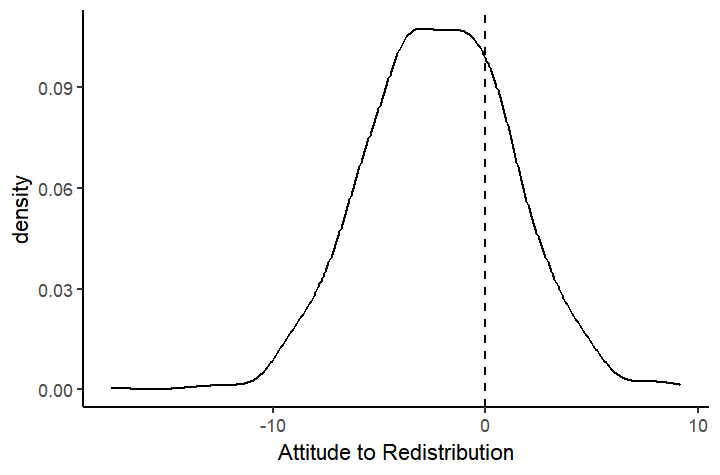
\includegraphics[width=\maxwidth]{figure/predictions3-1} 

\end{knitrout}
\end{multicols}
\end{frame}

\begin{frame}
\frametitle{7. Predictions from Regressions}
\begin{itemize}
\item The regression model matters because the wrong model makes non-sensical predictions
\item Consider a binary outcome: $Gender_i = \alpha + \beta Income_i + \epsilon_i$
\item Compare the OLS and Logit regression tables:
\end{itemize}
\begin{multicols}{2}

% Table created by stargazer v.5.2.2 by Marek Hlavac, Harvard University. E-mail: hlavac at fas.harvard.edu
% Date and time: Thu, Mar 07, 2019 - 8:44:04 AM
\begin{table}[!htbp] \centering 
  \caption{} 
  \label{} 
\tiny 
\begin{tabular}{@{\extracolsep{1pt}}lc} 
\\[-1.8ex]\hline 
\hline \\[-1.8ex] 
 & \multicolumn{1}{c}{\textit{Dependent variable:}} \\ 
\cline{2-2} 
\\[-1.8ex] & as.numeric(as.character(gender)) \\ 
\hline \\[-1.8ex] 
 income & 0.0003$^{***}$ (0.00001) \\ 
  Constant & $-$0.696$^{***}$ (0.066) \\ 
 \hline \\[-1.8ex] 
Observations & 1,000 \\ 
\hline 
\hline \\[-1.8ex] 
\textit{Note:}  & \multicolumn{1}{r}{$^{*}$p$<$0.1; $^{**}$p$<$0.05; $^{***}$p$<$0.01} \\ 
\end{tabular} 
\end{table} 

\columnbreak

% Table created by stargazer v.5.2.2 by Marek Hlavac, Harvard University. E-mail: hlavac at fas.harvard.edu
% Date and time: Thu, Mar 07, 2019 - 8:44:05 AM
\begin{table}[!htbp] \centering 
  \caption{} 
  \label{} 
\tiny 
\begin{tabular}{@{\extracolsep{1pt}}lc} 
\\[-1.8ex]\hline 
\hline \\[-1.8ex] 
 & \multicolumn{1}{c}{\textit{Dependent variable:}} \\ 
\cline{2-2} 
\\[-1.8ex] & as.numeric(as.character(gender)) \\ 
\hline \\[-1.8ex] 
 income & 0.001$^{***}$ (0.0001) \\ 
  Constant & $-$6.360$^{***}$ (0.457) \\ 
 \hline \\[-1.8ex] 
Observations & 1,000 \\ 
\hline 
\hline \\[-1.8ex] 
\textit{Note:}  & \multicolumn{1}{r}{$^{*}$p$<$0.1; $^{**}$p$<$0.05; $^{***}$p$<$0.01} \\ 
\end{tabular} 
\end{table} 

\end{multicols}
\end{frame}

\begin{frame}
\frametitle{7. Predictions from Regressions}
\begin{itemize}
\item The regression model matters because the wrong model makes non-sensical predictions
\item Consider a binary outcome: $Gender_i = \alpha + \beta Income_i + \epsilon_i$
\item Compare the OLS and Logit \textbf{predictions} of gender for an income of R\$3000:
\end{itemize}
\begin{multicols}{2}
\begin{knitrout}
\definecolor{shadecolor}{rgb}{0.969, 0.969, 0.969}\color{fgcolor}
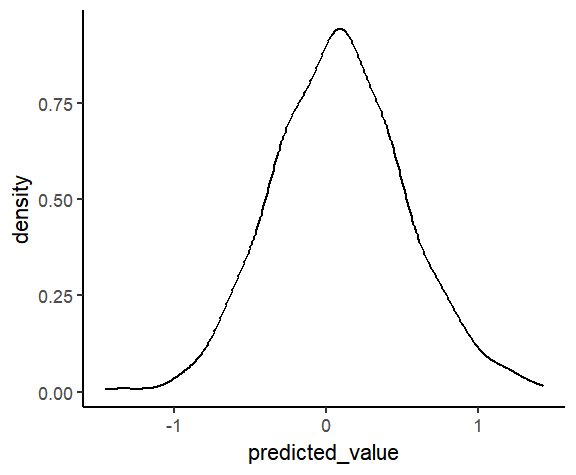
\includegraphics[width=\maxwidth]{figure/preds_1_ols_chart-1} 

\end{knitrout}
\columnbreak
\begin{knitrout}
\definecolor{shadecolor}{rgb}{0.969, 0.969, 0.969}\color{fgcolor}
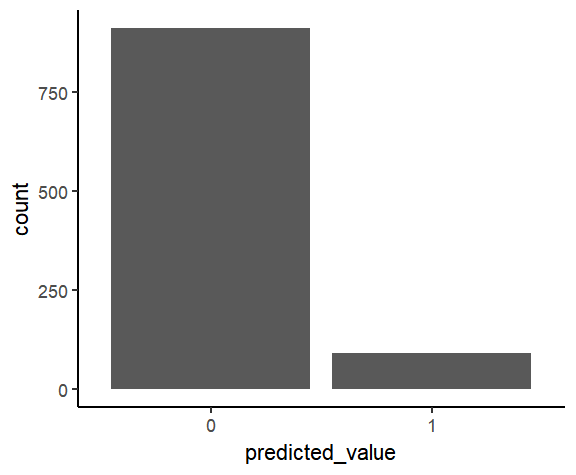
\includegraphics[width=\maxwidth]{figure/preds_1_logit_chart-1} 

\end{knitrout}
\end{multicols}
\end{frame}

\section{What Does Regression NOT Do?}

\begin{frame}
\frametitle{What Does Regression NOT Do?}
\begin{itemize}
\item Remember, regression is just fancy correlation
\item Even after following all this guidance, Regression does NOT:
\begin{enumerate}
\item \textit{Explain} anything
\item Make bad data better
\item Tell you which model is 'best'
\item Guarantee you are making sensible comparisons
\end{enumerate}
\item These all require \textbf{research design}, \textbf{theory} and \textbf{assumptions}
\end{itemize}
\end{frame}

\begin{frame}
\frametitle{What Does Regression NOT Do?}
\begin{itemize}
\item \textbf{Correlation is not causation}
\pause
\begin{itemize}
\item If we look hard enough we can always find correlations
\pause
\item By chance...
\pause
\item Due to complex social patterns...
\pause
\item But we cannot conclude that $D$ causes or explains $Y$
\pause
\end{itemize}
\item \textit{More} data will not help
\pause
\item The problem is the \textit{type} of data; it does not allow us to answer the causal question 
\end{itemize}
\end{frame}

\setbeamercolor{background canvas}{bg=}
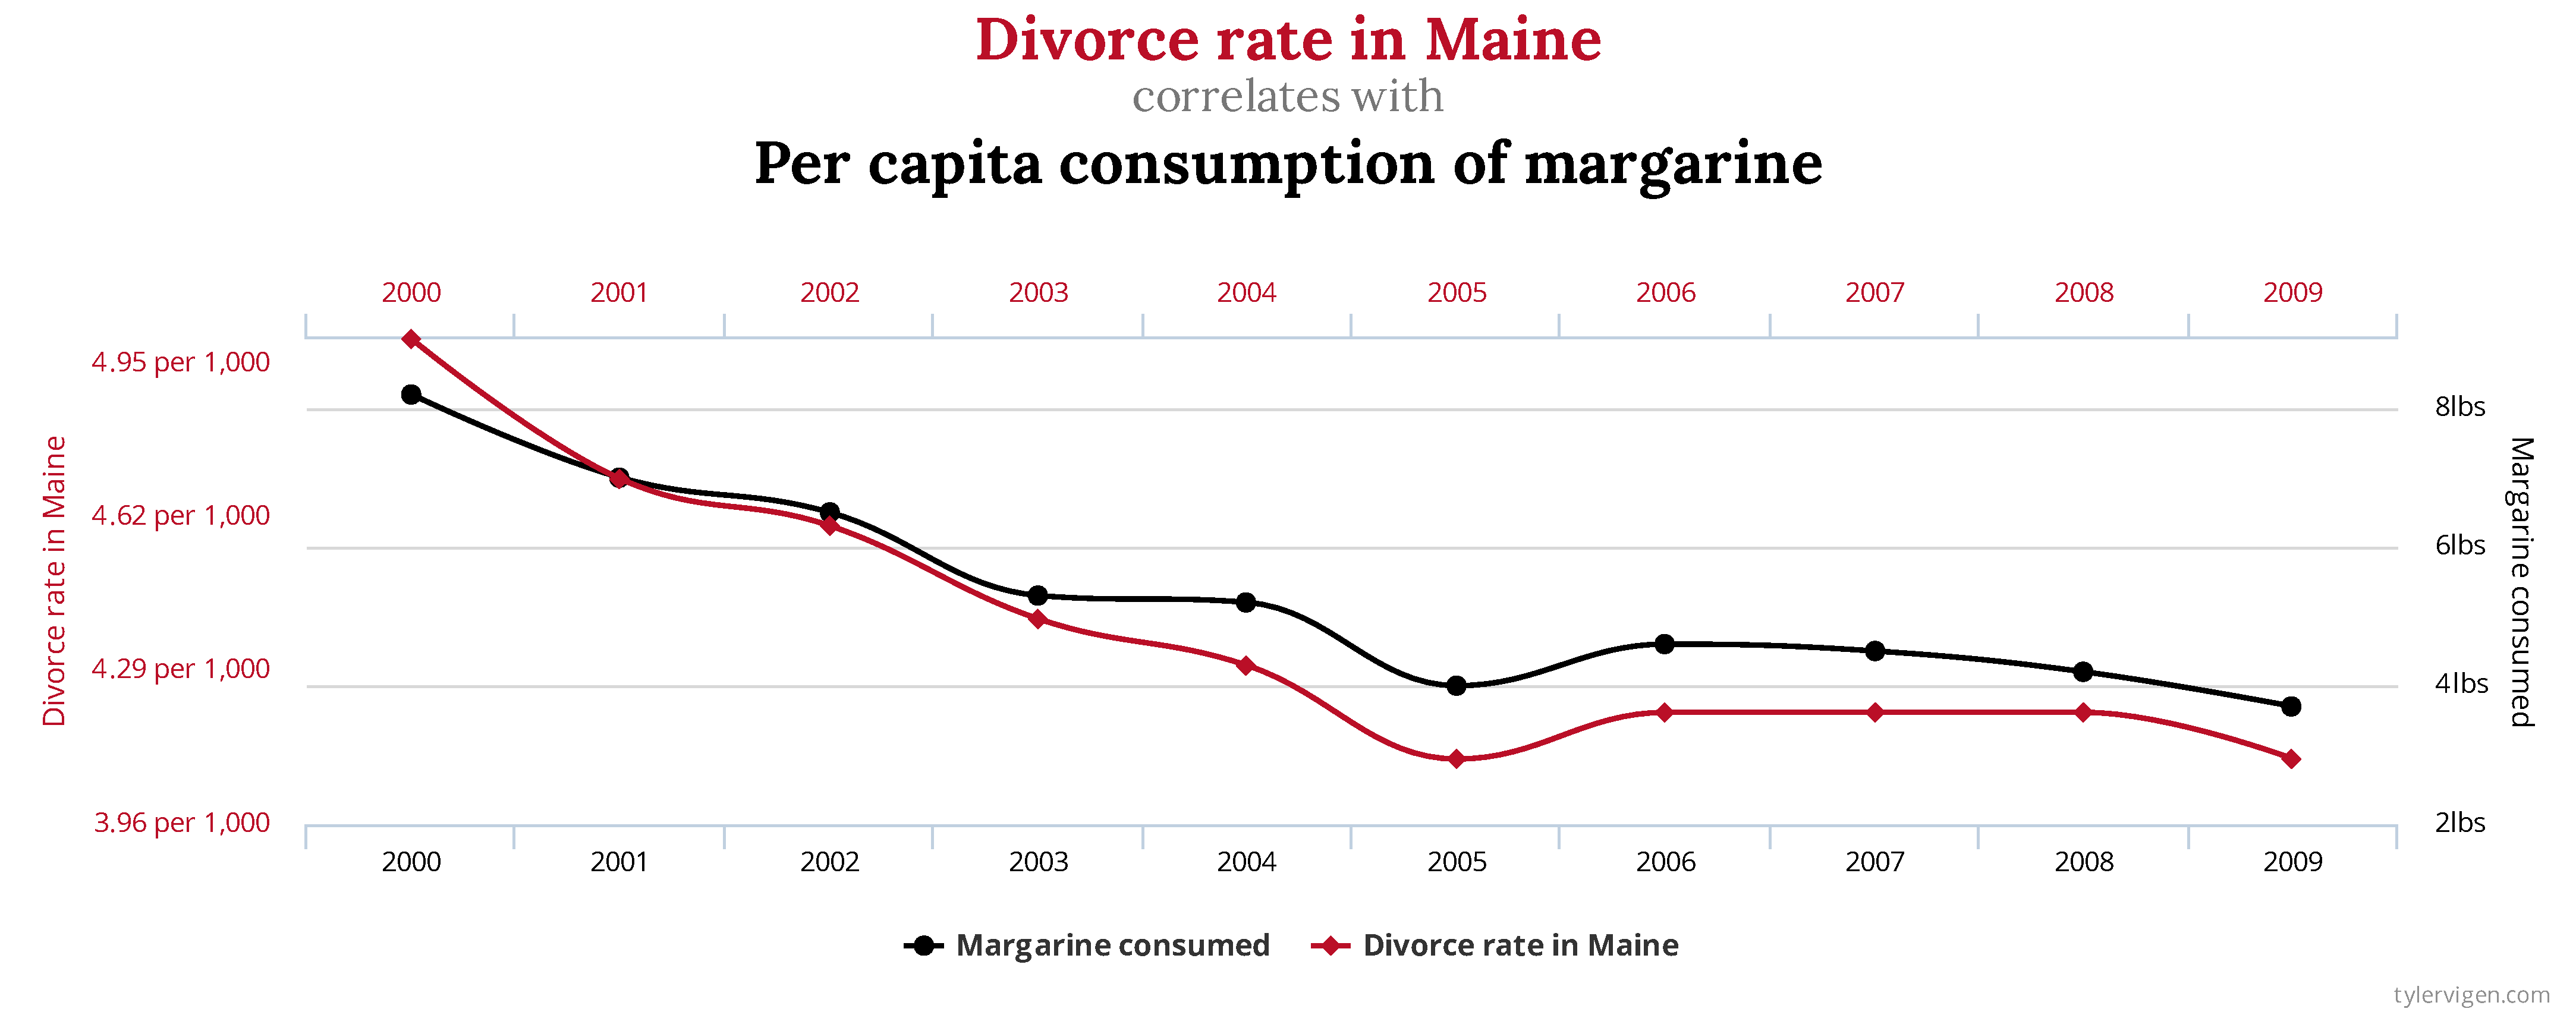
\includepdf[pages={1}]{chart_1.pdf}

\setbeamercolor{background canvas}{bg=}
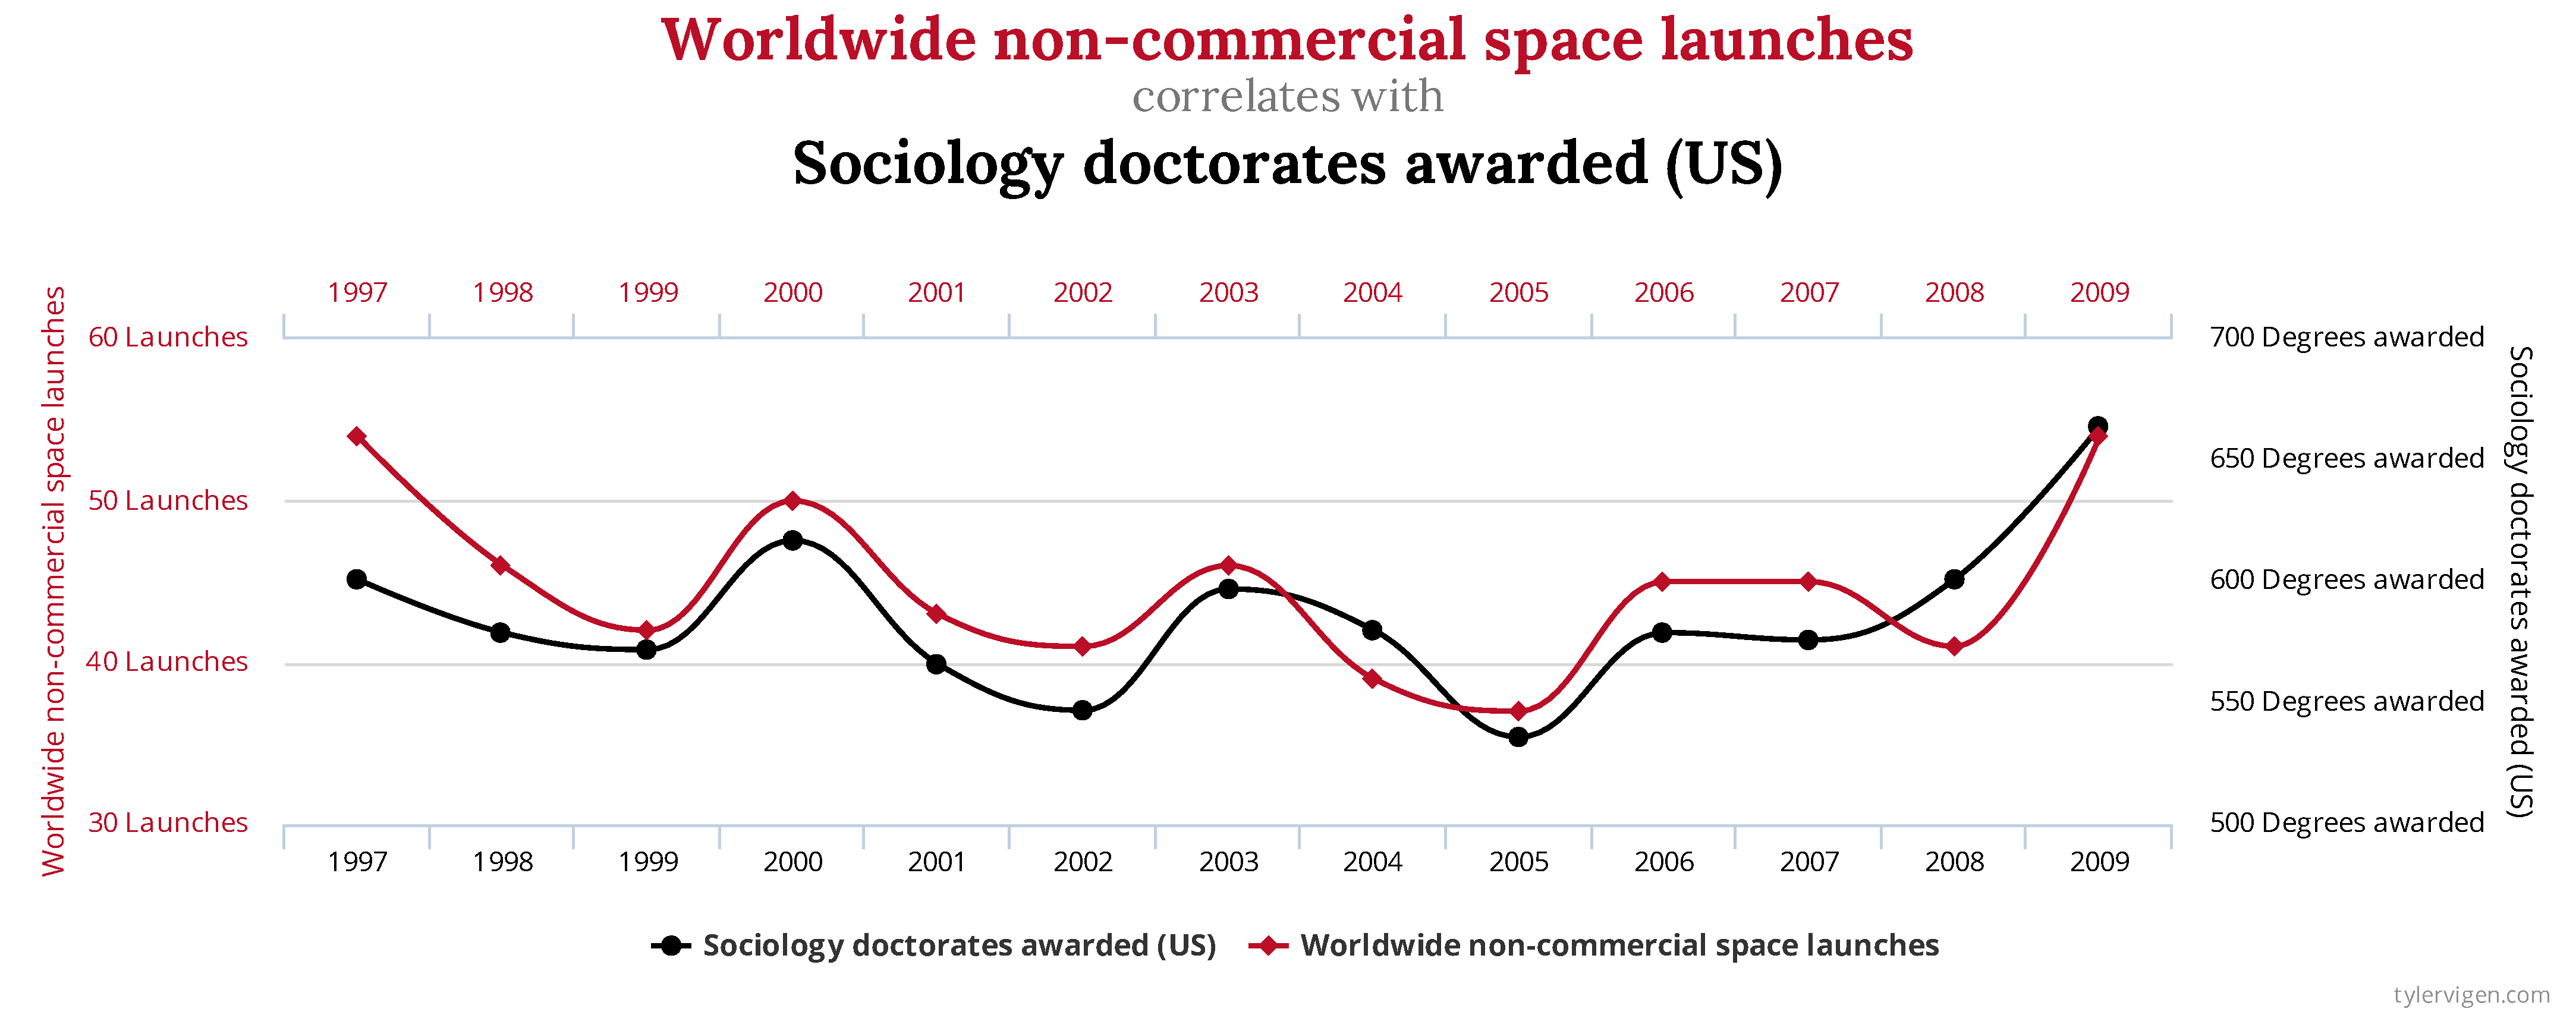
\includepdf[pages={1}]{chart_2.pdf}

\setbeamercolor{background canvas}{bg=}
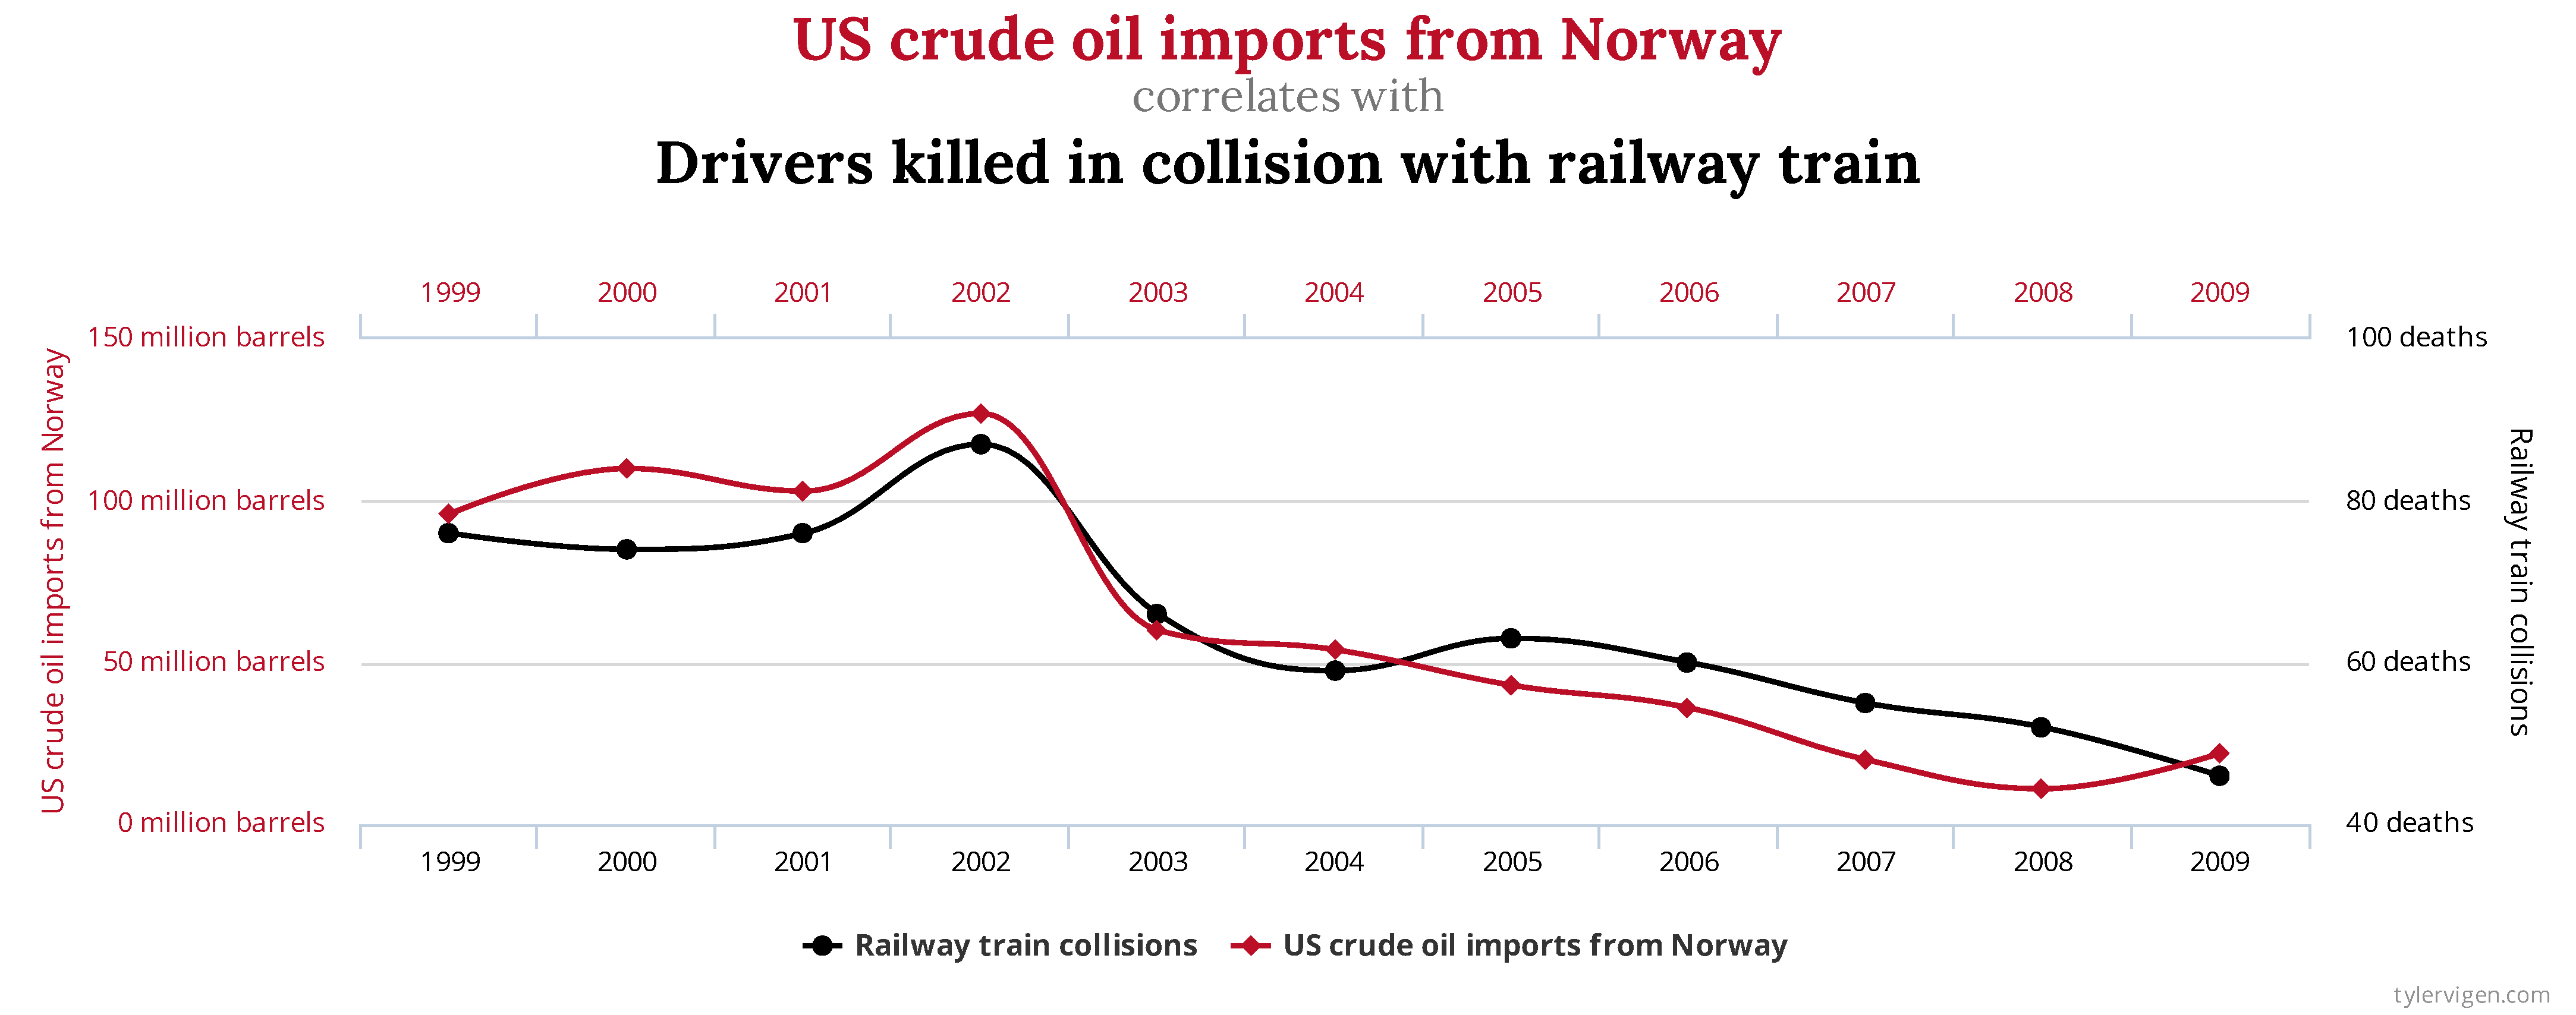
\includepdf[pages={1}]{chart_3.pdf}

\setbeamercolor{background canvas}{bg=}
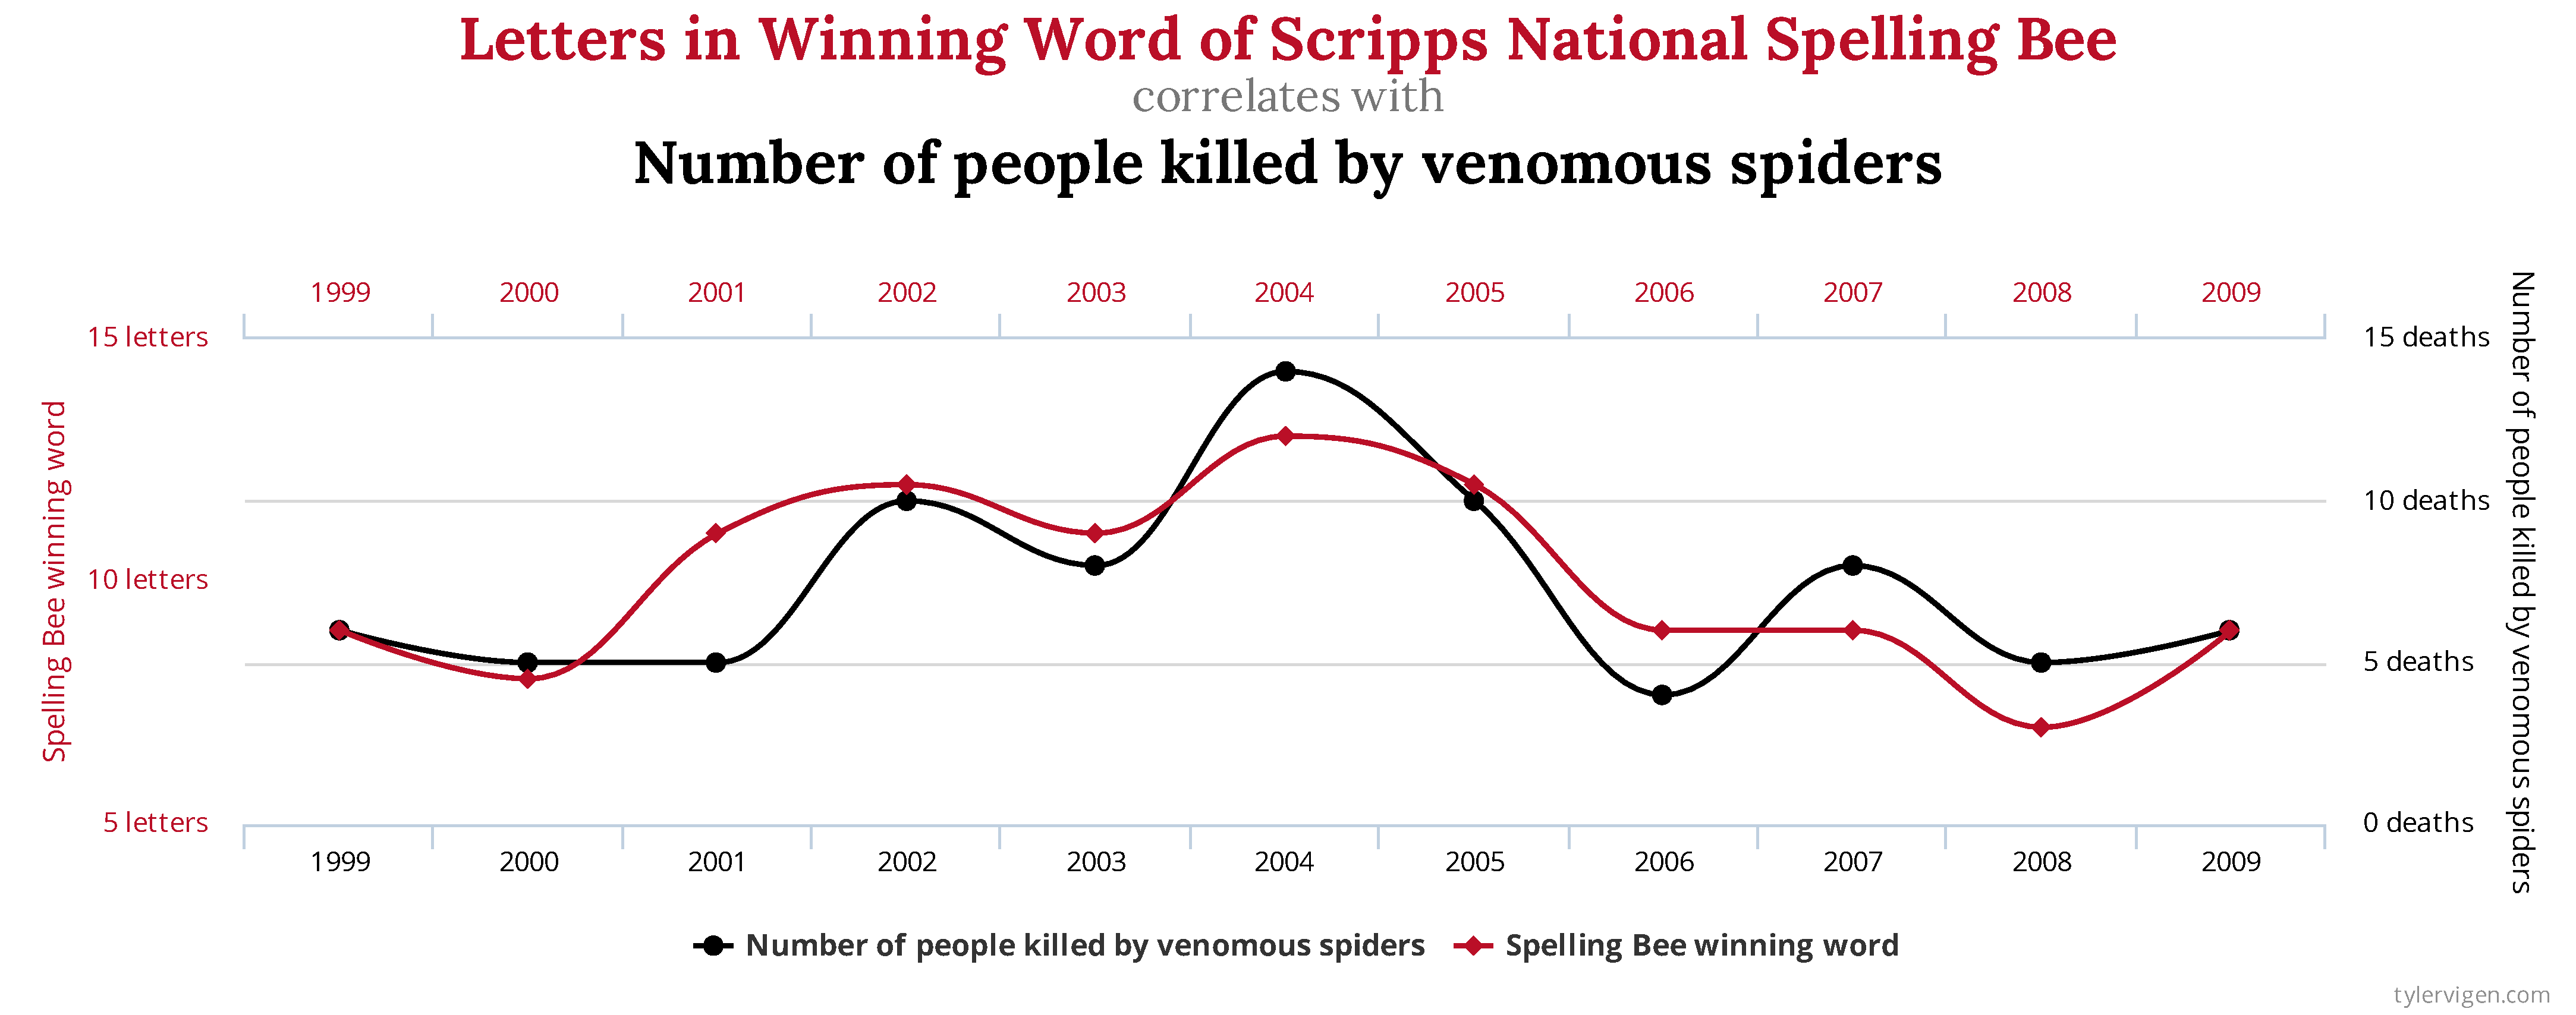
\includepdf[pages={1}]{chart_4.pdf}

\setbeamercolor{background canvas}{bg=}
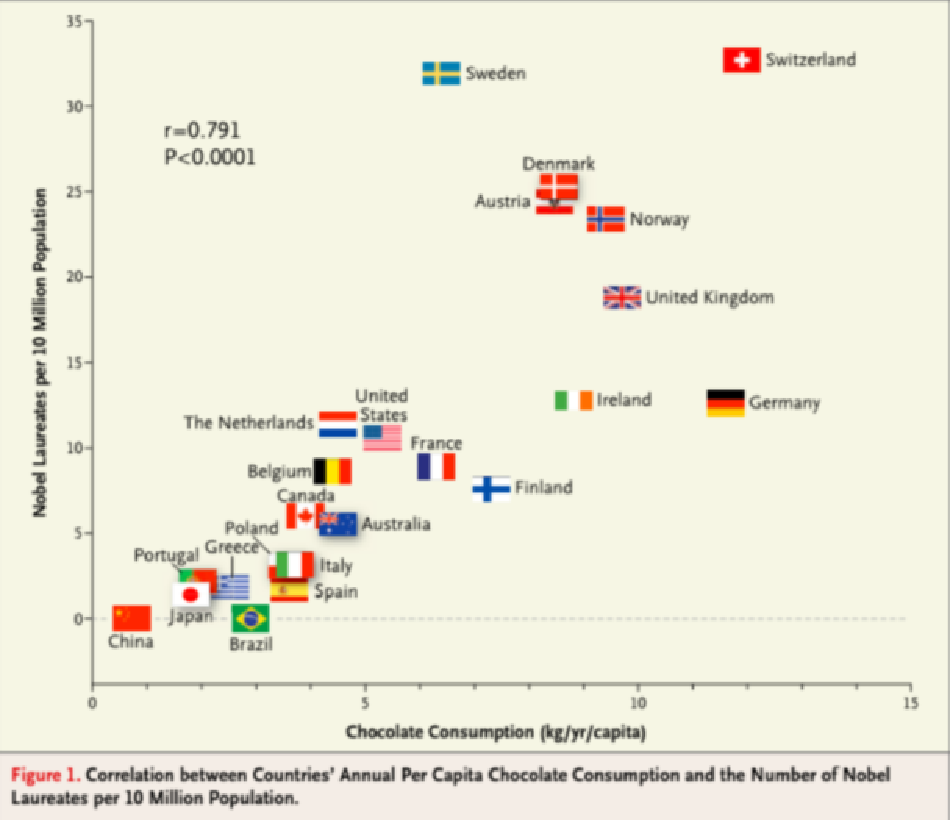
\includepdf[pages={1}]{Chocolate.pdf}

\begin{frame}
\frametitle{What Does Regression NOT Do?}
\begin{itemize}
\item Lots of things can go 'wrong' with regression:
\begin{enumerate}
\item Omitted Variable Bias
\item Reverse Causation
\item Selection Bias
\item Measurement Bias
\item Lack of Overlap, Model Dependence
\end{enumerate}
\end{itemize}
\end{frame}

\begin{frame}
\frametitle{1. Omitted Variable Bias}
\begin{knitrout}
\definecolor{shadecolor}{rgb}{0.969, 0.969, 0.969}\color{fgcolor}
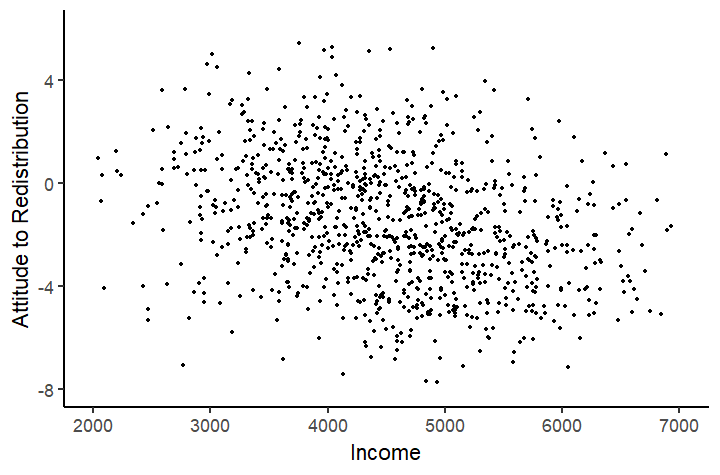
\includegraphics[width=\maxwidth]{figure/confound3b-1} 

\end{knitrout}
\end{frame}

\begin{frame}
\frametitle{1. Omitted Variable Bias}
\begin{knitrout}
\definecolor{shadecolor}{rgb}{0.969, 0.969, 0.969}\color{fgcolor}
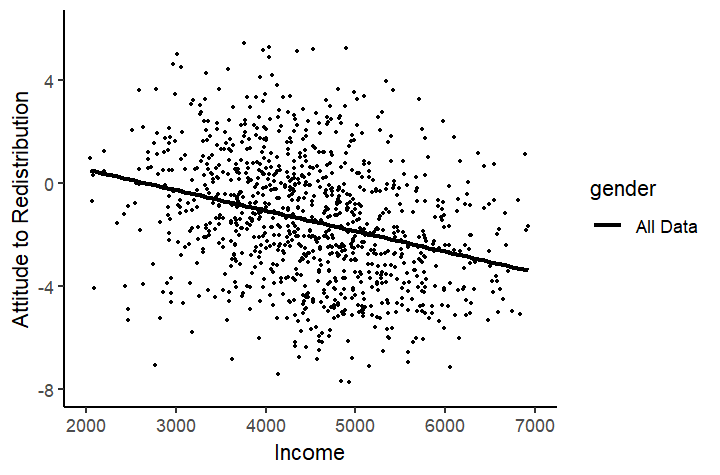
\includegraphics[width=\maxwidth]{figure/confound3c-1} 

\end{knitrout}
\end{frame}

\begin{frame}
\frametitle{1. Omitted Variable Bias}
\begin{knitrout}
\definecolor{shadecolor}{rgb}{0.969, 0.969, 0.969}\color{fgcolor}
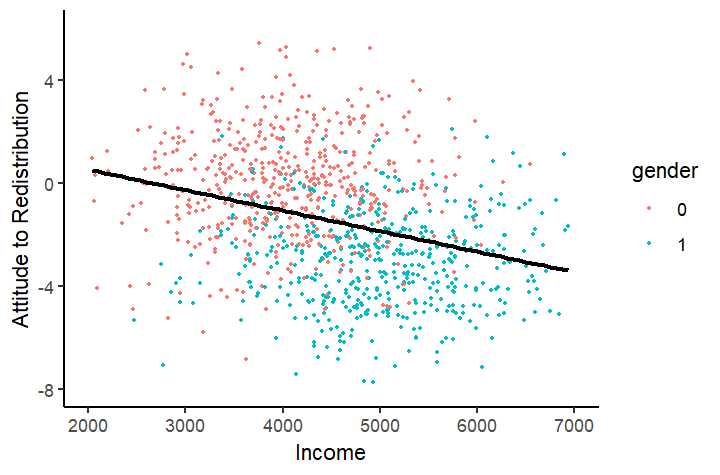
\includegraphics[width=\maxwidth]{figure/confound2-1} 

\end{knitrout}
\end{frame}


\begin{frame}
\frametitle{1. Omitted Variable Bias}
\begin{knitrout}
\definecolor{shadecolor}{rgb}{0.969, 0.969, 0.969}\color{fgcolor}
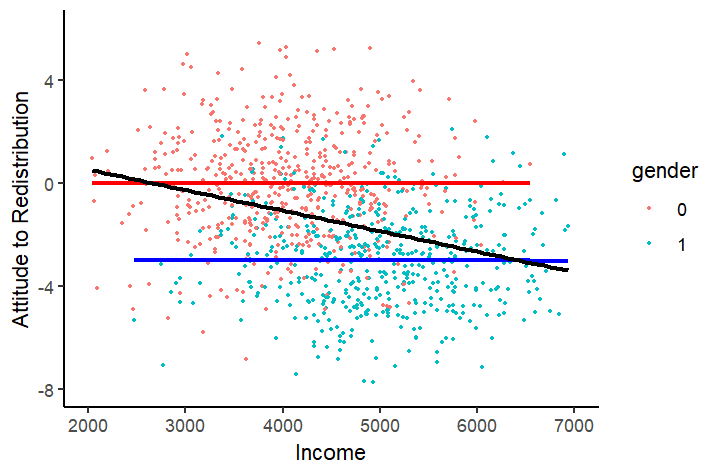
\includegraphics[width=\maxwidth]{figure/confound3-1} 

\end{knitrout}
\end{frame}

\begin{frame}
\frametitle{2. Reverse Causation}
\begin{itemize}
\item Significant regression coefficients just reflect the values in our dataset moving together
\pause
\item Does the 'direction' of regression  matter? I.e. Does regression treat $X$ and $Y$ differently?
\pause
\item Yes! 
\begin{multicols}{2}

% Table created by stargazer v.5.2.2 by Marek Hlavac, Harvard University. E-mail: hlavac at fas.harvard.edu
% Date and time: Wed, Mar 06, 2019 - 12:10:54 PM
\begin{table}[!htbp] \centering 
  \caption{} 
  \label{} 
\tiny 
\begin{tabular}{@{\extracolsep{1pt}}lc} 
\\[-1.8ex]\hline 
\hline \\[-1.8ex] 
 & \multicolumn{1}{c}{\textit{Dependent variable:}} \\ 
\cline{2-2} 
\\[-1.8ex] & redist \\ 
\hline \\[-1.8ex] 
 income & $-$0.011 (0.029) \\ 
  gender1 & $-$1.201$^{***}$ (0.058) \\ 
  Constant & 0.589$^{***}$ (0.038) \\ 
 \hline \\[-1.8ex] 
Observations & 1,000 \\ 
\hline 
\hline \\[-1.8ex] 
\textit{Note:}  & \multicolumn{1}{r}{$^{*}$p$<$0.1; $^{**}$p$<$0.05; $^{***}$p$<$0.01} \\ 
\end{tabular} 
\end{table} 

\columnbreak

% Table created by stargazer v.5.2.2 by Marek Hlavac, Harvard University. E-mail: hlavac at fas.harvard.edu
% Date and time: Wed, Mar 06, 2019 - 12:10:55 PM
\begin{table}[!htbp] \centering 
  \caption{} 
  \label{} 
\tiny 
\begin{tabular}{@{\extracolsep{1pt}}lc} 
\\[-1.8ex]\hline 
\hline \\[-1.8ex] 
 & \multicolumn{1}{c}{\textit{Dependent variable:}} \\ 
\cline{2-2} 
\\[-1.8ex] & income \\ 
\hline \\[-1.8ex] 
 redist & $-$0.013 (0.034) \\ 
  gender1 & 0.993$^{***}$ (0.069) \\ 
  Constant & $-$0.487$^{***}$ (0.043) \\ 
 \hline \\[-1.8ex] 
Observations & 1,000 \\ 
\hline 
\hline \\[-1.8ex] 
\textit{Note:}  & \multicolumn{1}{r}{$^{*}$p$<$0.1; $^{**}$p$<$0.05; $^{***}$p$<$0.01} \\ 
\end{tabular} 
\end{table} 

\end{multicols}
\item Remember, regression measures the \textit{vertical} (not diagonal) distances to the regression line
\begin{itemize}
\item It minimizes the prediction errors for $Y$
\end{itemize}
\item But that doesn't mean it identifies the direction of causation!
\end{itemize}
\end{frame}

\begin{frame}
\frametitle{3. Selection Bias}
\begin{itemize}
\item There are four selection risks:
\begin{enumerate}
\item \textbf{Selection into existence}
\item \textbf{Selection into survival}
\item \textbf{Selection into the dataset}
\item \textbf{Selection into treatment}
\end{enumerate}
\item In each case, we don't see the \textit{full} relationship between $X$ and $Y$
\item So our regression estimates are biased
\end{itemize}
\end{frame}

\begin{frame}
\frametitle{3. Selection Bias}
\begin{itemize}
\item Imagine we do not see 'rich' units with high income (above R\$4000)
\end{itemize}
\begin{knitrout}
\definecolor{shadecolor}{rgb}{0.969, 0.969, 0.969}\color{fgcolor}
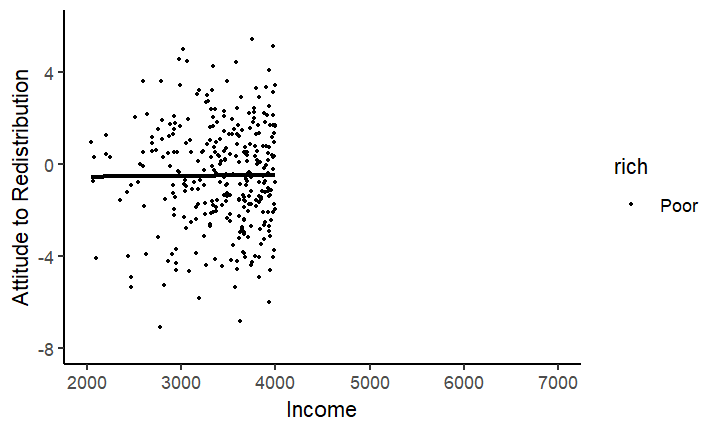
\includegraphics[width=\maxwidth]{figure/selection1-1} 

\end{knitrout}
\end{frame}

\begin{frame}
\frametitle{3. Selection Bias}
\begin{itemize}
\item Imagine we do not see 'rich' units with high income (above R\$4000)
\end{itemize}
\begin{knitrout}
\definecolor{shadecolor}{rgb}{0.969, 0.969, 0.969}\color{fgcolor}
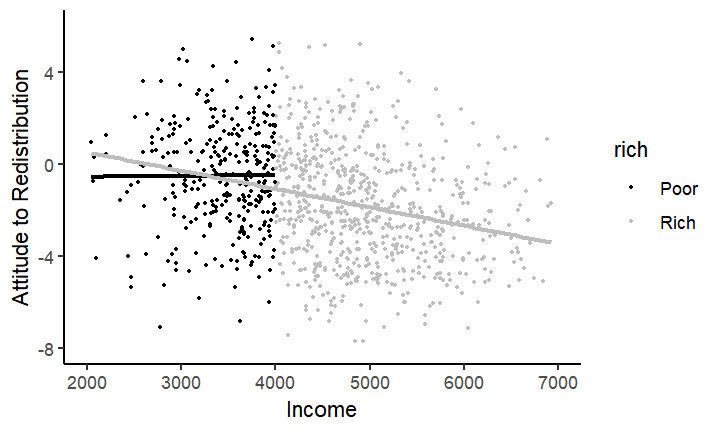
\includegraphics[width=\maxwidth]{figure/selection2-1} 

\end{knitrout}
\end{frame}

\begin{frame}
\frametitle{3. Selection Bias}
\begin{itemize}
\item There are four selection risks:
\begin{enumerate}
\item \textbf{Selection into existence:}
\begin{itemize}
\item Where do units (eg. political parties) come from?
\item Probably only parties that have a chance of success are formed
\item Does forming a party cause electoral success? Not for most people!
\end{itemize}
\end{enumerate}
\end{itemize}
\end{frame}

\begin{frame}
\frametitle{3. Selection Bias}
\begin{itemize}
\item There are four selection risks:
\begin{enumerate}
\setcounter{enumi}{1}
\item \textbf{Selection into survival:}
\begin{itemize}
\item Certain types of units disappear, so the units we see don't tell the full story
\end{itemize}
\end{enumerate}
\end{itemize}
\begin{multicols}{2}
\includegraphics[scale=0.25]{Bombers.pdf}
\columnbreak
\begin{itemize}
\item Where would additional armour protect bombers?
\item Returned bombers got hit
\item But we do not know where \textit{bombers that did not return} got hit
\end{itemize}
\end{multicols}
\end{frame}

\begin{frame}
\frametitle{3. Selection Bias}
\begin{itemize}
\item There are four selection risks:
\begin{enumerate}
\setcounter{enumi}{2}
\item \textbf{Selection into the dataset:}
\begin{itemize}
\item Our dataset may not be representative
\item Only units with particular values of $X$ and $Y$ enter the dataset
\item Eg. If survey respondents who refuse are different from those who respond
\end{itemize}
\end{enumerate}
\end{itemize}
\end{frame}

\begin{frame}
\frametitle{3. Selection Bias}
\begin{itemize}
\item There are four selection risks:
\begin{enumerate}
\setcounter{enumi}{3}
\item \textbf{Selection into treatment:}
\begin{itemize}
\item All units are in our dataset, but they \textit{choose} their treatment value
\item Who chooses treatment? Those with the most to benefit, i.e. depending on $Y$!
\item Applying treatment to the others would probably have a very different effect
\end{itemize}
\end{enumerate}
\end{itemize}
\end{frame}

\begin{frame}
\frametitle{4. Measurement Bias}
\begin{itemize}
\item What happens if we measure our variables wrongly?
\footnotesize
\begin{table}[htbp]
  \centering
  \caption{Effects of Measurement Error}
    \begin{tabular}{|l|l|p{4cm}|}
    \hline
          & Measured with Bias & Measured with Random Noise \bigstrut\\
    \hline
    Outcome Variable & Effect biased & No bias but wider standard errors \bigstrut\\
    \hline
    Treatment Variable & Effect biased & Effect biased to zero \bigstrut\\
    \hline
    \end{tabular}%
  \label{tab:addlabel}%
\end{table}%
\normalsize
\end{itemize}
\end{frame}

\begin{frame}
\frametitle{4. Measurement Bias}
\begin{itemize}
\item What happens if we measure our variables wrongly?
\item No extra noise:
\end{itemize}
\begin{multicols}{2}
\begin{knitrout}
\definecolor{shadecolor}{rgb}{0.969, 0.969, 0.969}\color{fgcolor}
\includegraphics[width=\maxwidth]{figure/measure2-1} 

\end{knitrout}
\columnbreak

\begin{table}[!htbp] \centering 
  \caption{} 
  \label{} 
\tiny 
\begin{tabular}{@{\extracolsep{1pt}}lc} 
\\[-1.8ex]\hline 
\hline \\[-1.8ex] 
 & \multicolumn{1}{c}{\textit{Dependent variable:}} \\ 
\cline{2-2} 
\\[-1.8ex] & redist \\ 
\hline \\[-1.8ex] 
 income & $-$0.818$^{***}$ (0.078) \\ 
  Constant & 2.235$^{***}$ (0.361) \\ 
 \hline \\[-1.8ex] 
Observations & 1,000 \\ 
\hline 
\hline \\[-1.8ex] 
\textit{Note:}  & \multicolumn{1}{r}{$^{*}$p$<$0.1; $^{**}$p$<$0.05; $^{***}$p$<$0.01} \\ 
\end{tabular} 
\end{table} 

\end{multicols}
\end{frame}

\begin{frame}
\frametitle{4. Measurement Bias}
\begin{itemize}
\item What happens if we measure our variables wrongly?
\item Noise in the \textbf{outcome variable}:
\end{itemize}
\begin{multicols}{2}
\begin{knitrout}
\definecolor{shadecolor}{rgb}{0.969, 0.969, 0.969}\color{fgcolor}
\includegraphics[width=\maxwidth]{figure/measure2b-1} 

\end{knitrout}
\columnbreak

\begin{table}[!htbp] \centering 
  \caption{} 
  \label{} 
\tiny 
\begin{tabular}{@{\extracolsep{1pt}}lc} 
\\[-1.8ex]\hline 
\hline \\[-1.8ex] 
 & \multicolumn{1}{c}{\textit{Dependent variable:}} \\ 
\cline{2-2} 
\\[-1.8ex] & redist \\ 
\hline \\[-1.8ex] 
 income & $-$0.831$^{***}$ (0.144) \\ 
  Constant & 2.272$^{***}$ (0.665) \\ 
 \hline \\[-1.8ex] 
Observations & 1,000 \\ 
\hline 
\hline \\[-1.8ex] 
\textit{Note:}  & \multicolumn{1}{r}{$^{*}$p$<$0.1; $^{**}$p$<$0.05; $^{***}$p$<$0.01} \\ 
\end{tabular} 
\end{table} 

\end{multicols}
\end{frame}

\begin{frame}
\frametitle{4. Measurement Bias}
\begin{itemize}
\item What happens if we measure our variables wrongly?
\item Noise in the \textbf{explanatory} variable:
\end{itemize}
\begin{multicols}{2}
\begin{knitrout}
\definecolor{shadecolor}{rgb}{0.969, 0.969, 0.969}\color{fgcolor}
\includegraphics[width=\maxwidth]{figure/measure2c-1} 

\end{knitrout}
\columnbreak

\begin{table}[!htbp] \centering 
  \caption{} 
  \label{} 
\tiny 
\begin{tabular}{@{\extracolsep{1pt}}lc} 
\\[-1.8ex]\hline 
\hline \\[-1.8ex] 
 & \multicolumn{1}{c}{\textit{Dependent variable:}} \\ 
\cline{2-2} 
\\[-1.8ex] & redist \\ 
\hline \\[-1.8ex] 
 income & $-$0.187$^{***}$ (0.037) \\ 
  Constant & $-$0.620$^{***}$ (0.183) \\ 
 \hline \\[-1.8ex] 
Observations & 1,000 \\ 
\hline 
\hline \\[-1.8ex] 
\textit{Note:}  & \multicolumn{1}{r}{$^{*}$p$<$0.1; $^{**}$p$<$0.05; $^{***}$p$<$0.01} \\ 
\end{tabular} 
\end{table} 

\end{multicols}
\end{frame}

\begin{frame}
\frametitle{5. Lack of Overlap}
\begin{itemize}
\item Regression normally helps us pick appropriate comparisons
\begin{itemize}
\item Eg. Comparing only among men, what is the effect of income on attitudes to redistribution? 
\end{itemize}
\item But what if there are no women with high income?
\item Regression \textit{creates} comparisons for us
\begin{itemize}
\item How? That's where the functional for of the regression comes in
\item A linear regression interpolates/extrapolates \textit{linearly} to 'create' comparison cases
\end{itemize}
\item Lack of overlap probably means we \textit{cannot} explain outcomes with this data
\end{itemize}
\end{frame}

\begin{frame}
\frametitle{5. Lack of Overlap}
\begin{knitrout}
\definecolor{shadecolor}{rgb}{0.969, 0.969, 0.969}\color{fgcolor}
\includegraphics[width=\maxwidth]{figure/overlap1-1} 

\end{knitrout}
\end{frame}

\begin{frame}
\frametitle{5. Lack of Overlap}
\begin{knitrout}
\definecolor{shadecolor}{rgb}{0.969, 0.969, 0.969}\color{fgcolor}
\includegraphics[width=\maxwidth]{figure/overlap2-1} 

\end{knitrout}
\end{frame}

\begin{frame}
\frametitle{5. Lack of Overlap}
\begin{knitrout}
\definecolor{shadecolor}{rgb}{0.969, 0.969, 0.969}\color{fgcolor}
\includegraphics[width=\maxwidth]{figure/overlap3-1} 

\end{knitrout}
\end{frame}

\begin{frame}
\frametitle{5. Lack of Overlap}
\begin{itemize}
\item With more than a few variables, lack of overlap is \textit{guaranteed}
\item 6 variables with 10 categories each = $10^6 = 1,000,000$ possibilities, and a sample of maybe 5,000?
\item Common datasets have 0\% counterfactuals present in the data (King 2006)
\begin{itemize}
\item How many 45 year-old female accountants with a PhD and a cat who live in Centro are there?
\item And we need some that are low-income and some that are high-income
\end{itemize}
\item A problem of \textbf{multi-dimensionality}
\item And of \textbf{model dependence} - our results depend on the functional form in our regression model
\end{itemize}
\end{frame}


% Stress - in prep for week 2 - that regression only buys you (conditional) correlation

%Chenage all examples to age-gender-income

\end{document}


%setwd('C:\\Users\\Jonny\\Google Drive\\Academic\\USP\\Class\\Week 1 - Intro\\Lecture Slides')
%knitr::knit("Slides_Wk1_intro_5.Rnw")
